\subsection{Identification}

\begin{frame}{Usual way to identify structures: Diffraction}
	\begin{columns}
	\column{0.5\textwidth}
	\def\svgwidth{\columnwidth}\input{xray.pdf_tex}
	\begin{itemize}
		\item Average over illuminated area
		\item Long ranged positional order
		\item Coherent orientation
	\end{itemize}
	\column{0.5\textwidth}
	\centering Quasi-crystal\\
	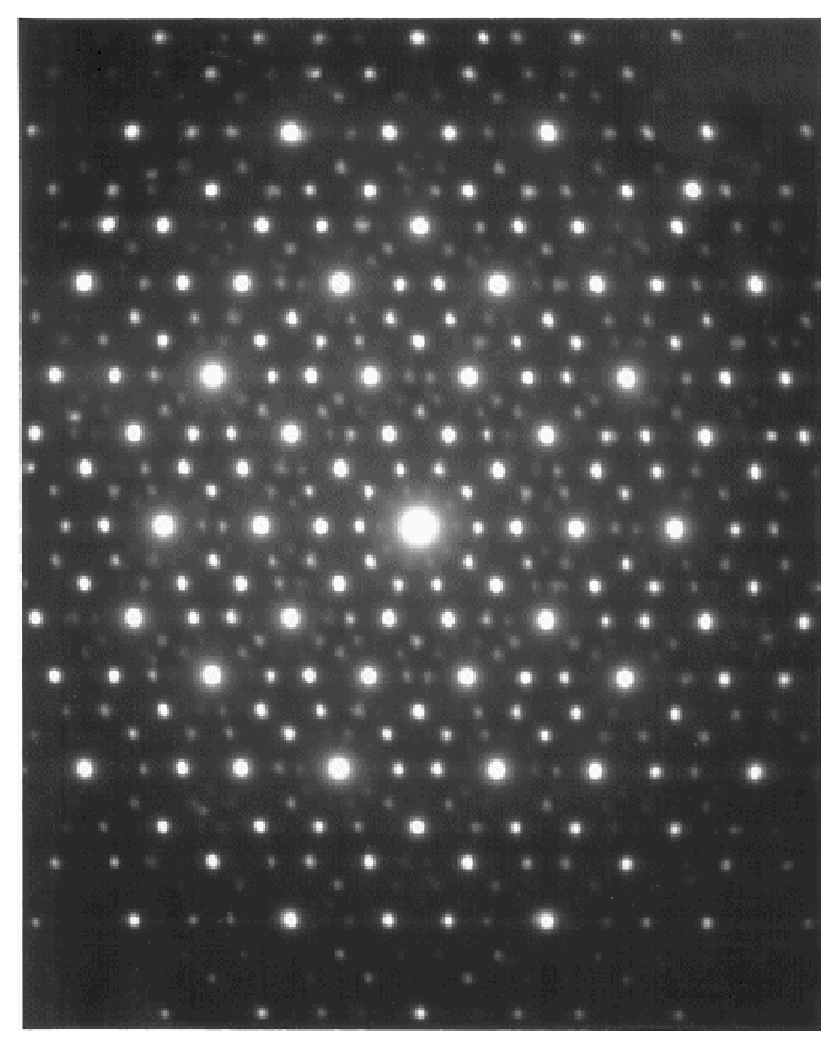
\includegraphics[width=\columnwidth]{diffraction_quasiX}
	\end{columns}
\end{frame}

\begin{frame}{Local symmetry}
	\begin{center}
	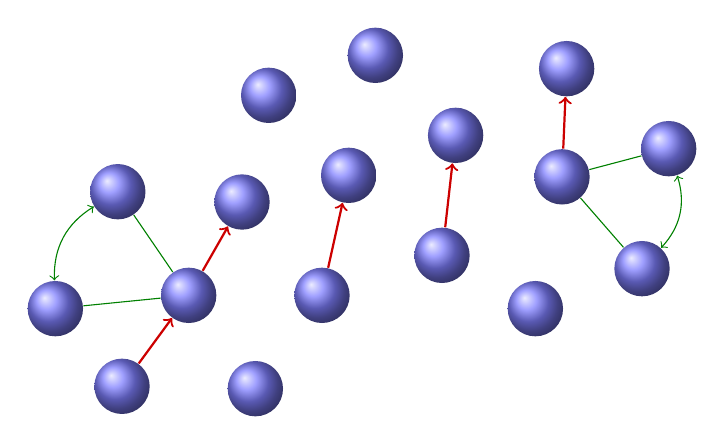
\begin{tikzpicture}[scale=0.3]
		\tikzset{particle/.style={circle, ball color=blue!50!white, inner sep=0, minimum size=2em}}
		\tikzset{ar/.style={->, draw=red!80!black, thick}}
		\node[particle] at (14.356, 47.436) (a) {};
		\node[particle] at (17.000, 52.387) (b) {};
		\node[particle] at (20.000, 48.000) (c) {};
		\node[particle] at (17.178, 44.149) (d) {};
		\node[particle] at (22.258, 51.951) (e) {};
		\node[particle] at (22.822, 44.049) (f) {};
		\node[particle] at (23.387, 56.467) (g) {};
		\node[particle] at (27.902, 58.160) (g1) {};
		\node[particle] at (26.773, 53.080) (h) {};
		\node[particle] at (25.644, 48.000) (i) {};
		\node[particle] at (31.300, 54.773) (j) {};
		\node[particle] at (30.724, 49.693) (k) {};
		\node[particle] at (36.000, 57.596) (k1) {};
		\node[particle] at (35.804, 53.016) (l) {};
		\node[particle] at (34.676, 47.436) (m) {};
		\node[particle] at (40.320, 54.209) (n) {};
		\node[particle] at (39.191, 49.129) (o) {};
		\path[ar] (d) edge (c);
		\path[ar] (c) edge (e);
		\path[ar] (i) edge (h);
		\path[ar] (k) edge (j);
		\path[ar] (l) edge (k1);
		\draw[green!50!black] (a) -- (c) -- (b);
		\path[green!50!black,<->] (a) edge [bend left] (b);
		\draw[green!50!black] (n) -- (l) -- (o);
		\path[green!50!black,<->] (n) edge [bend left] (o);
	\end{tikzpicture}
	\begin{itemize}
		\item The orientation changes $\Rightarrow$ No positional order
		\item The local angles stay the same $\Rightarrow$ Bond orientational order
	\end{itemize}
	\end{center}
\end{frame}

\begin{frame}{Local structures}
	\begin{center}\begin{tabular}{ccc}
	FCC & HCP & Icosahedron \\ 
	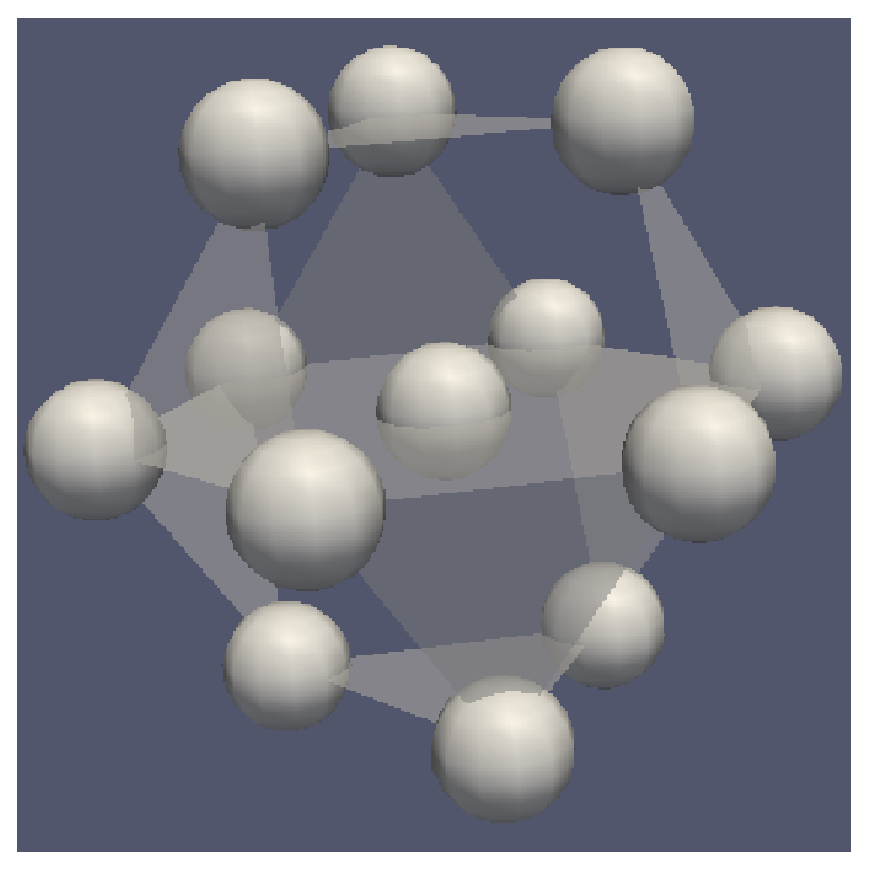
\includegraphics[width=0.27\textwidth]{fcc_13} & 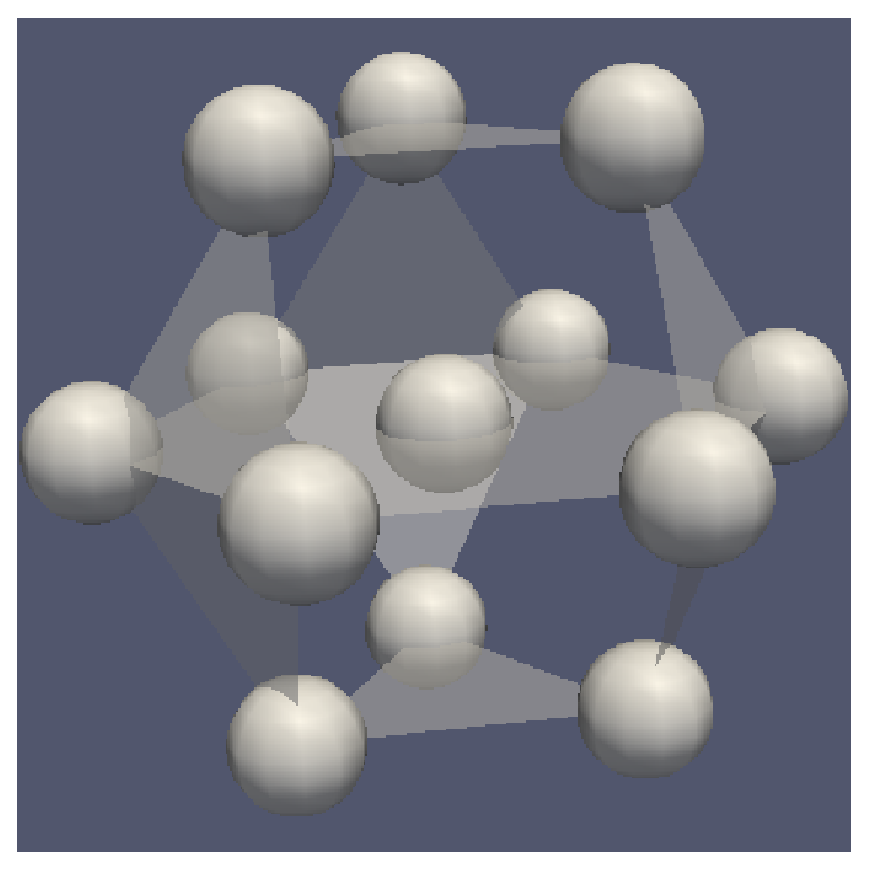
\includegraphics[width=0.27\textwidth]{hcp_13} & 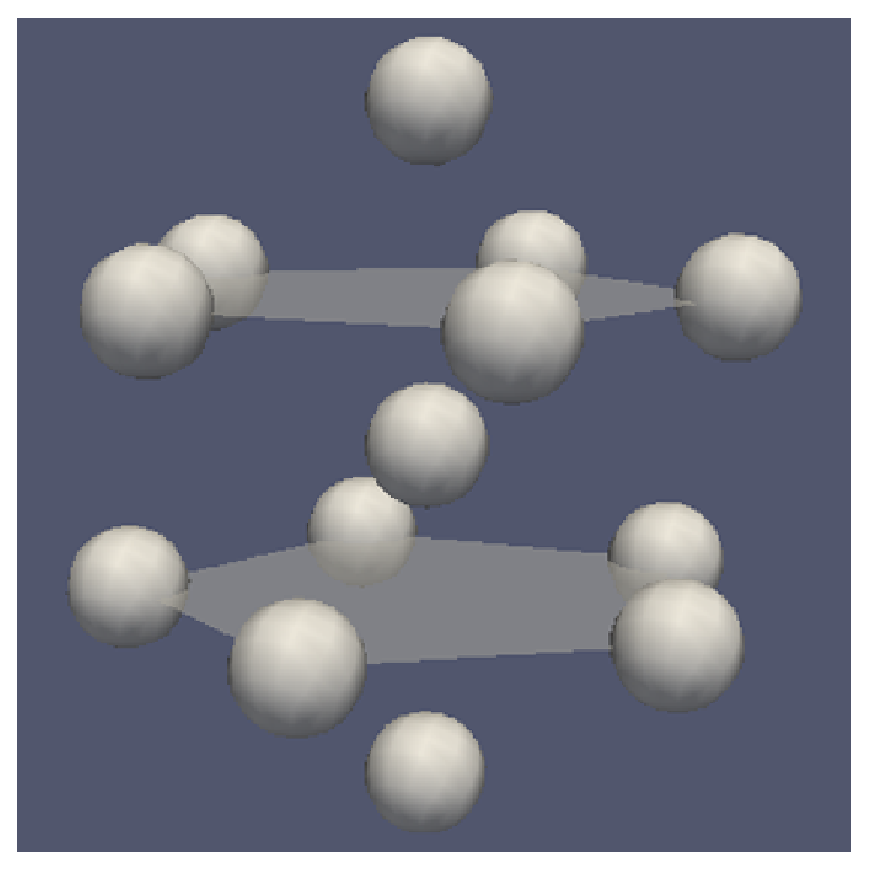
\includegraphics[width=0.27\textwidth]{ico_13}
	\end{tabular}
	\only<all:1>{\begin{tabular}{ccc}
	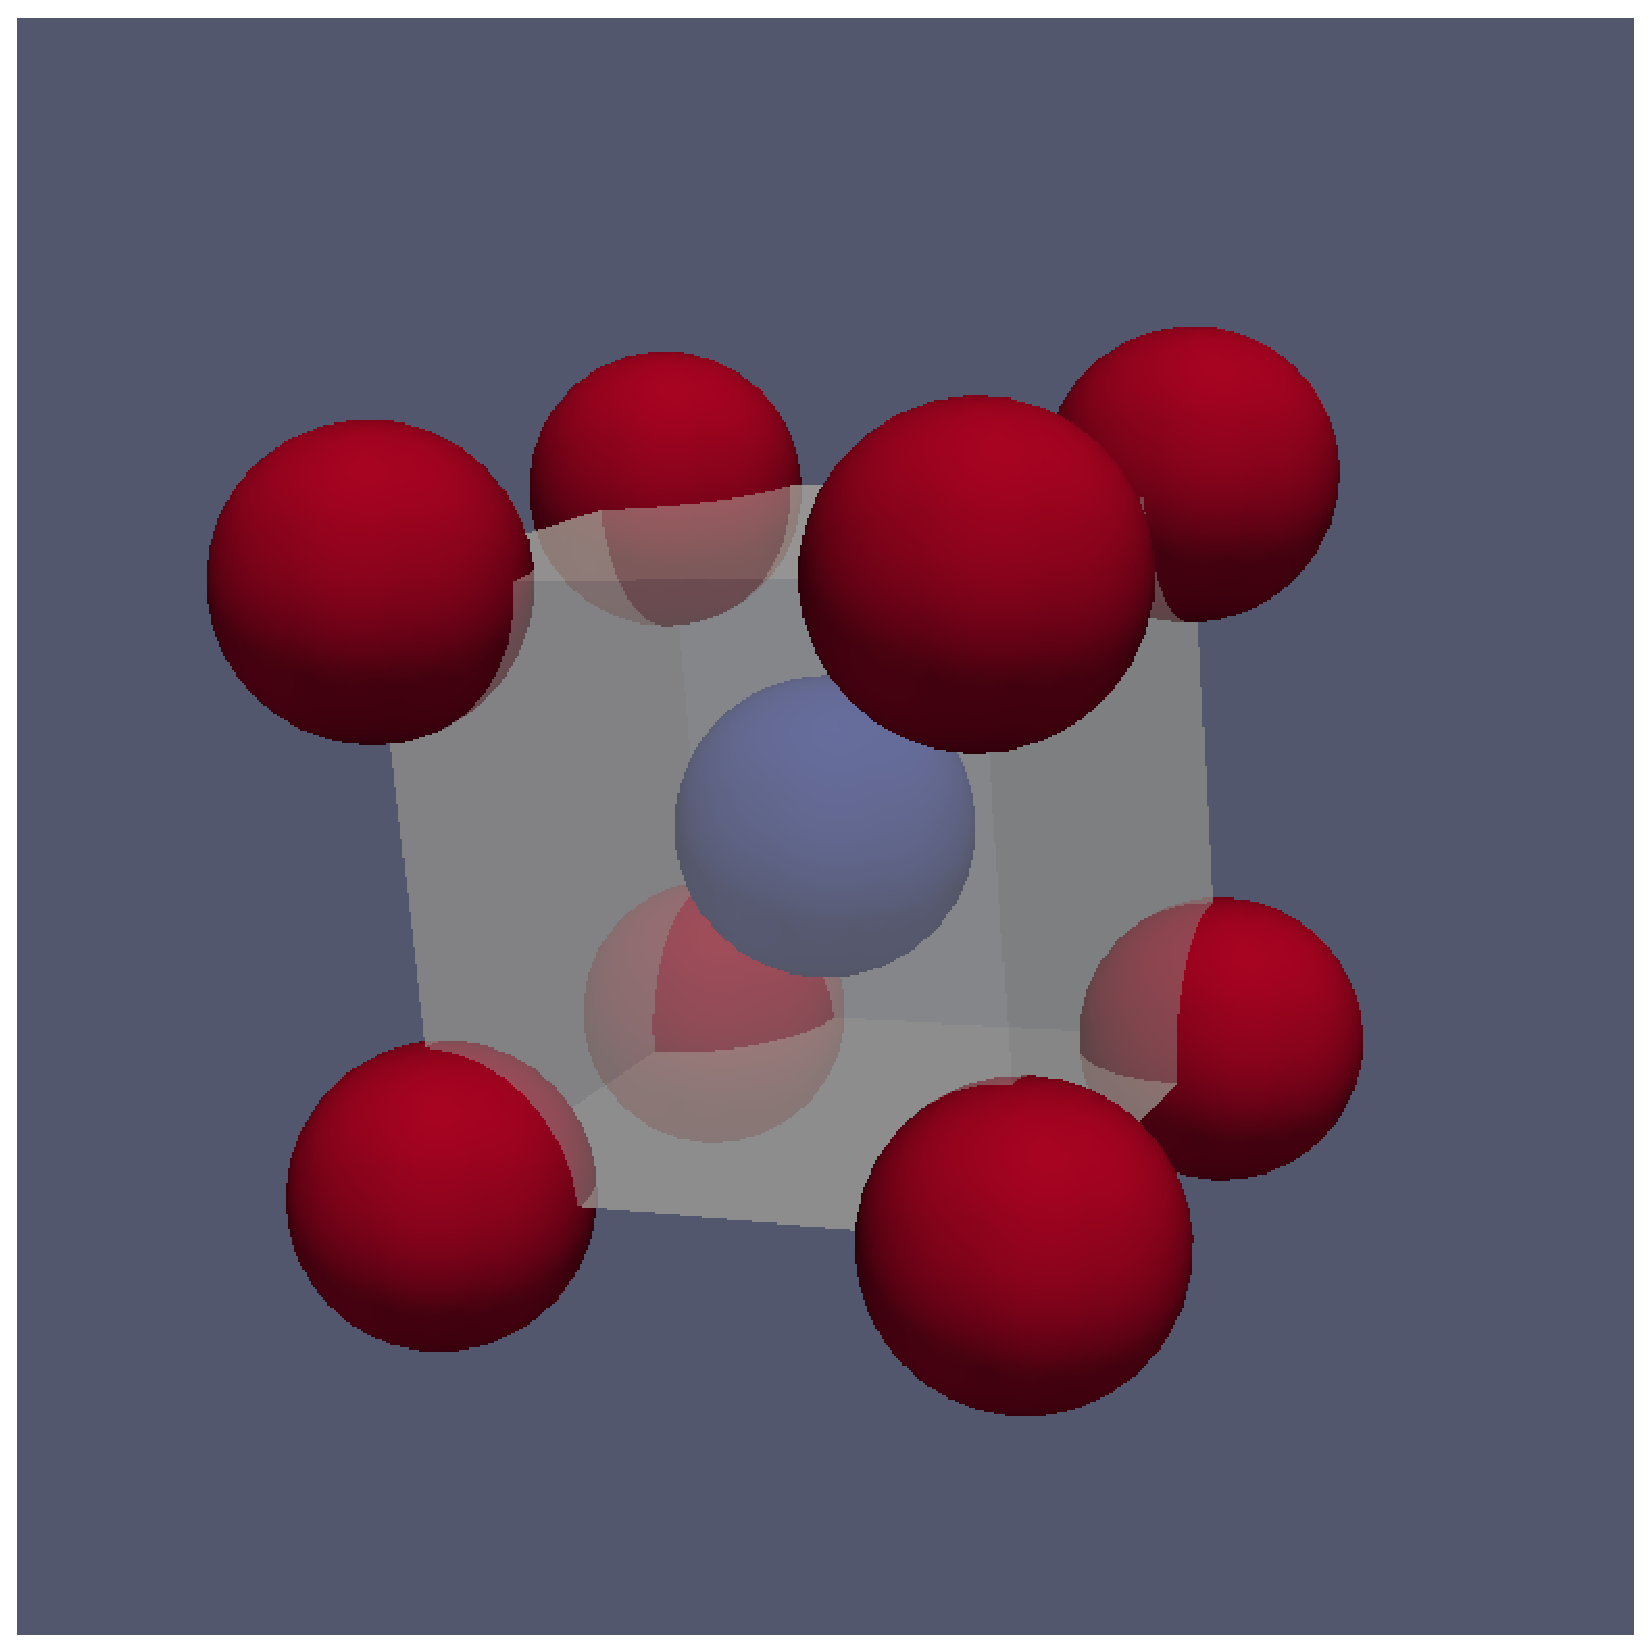
\includegraphics[width=0.27\textwidth]{bcc_9} & 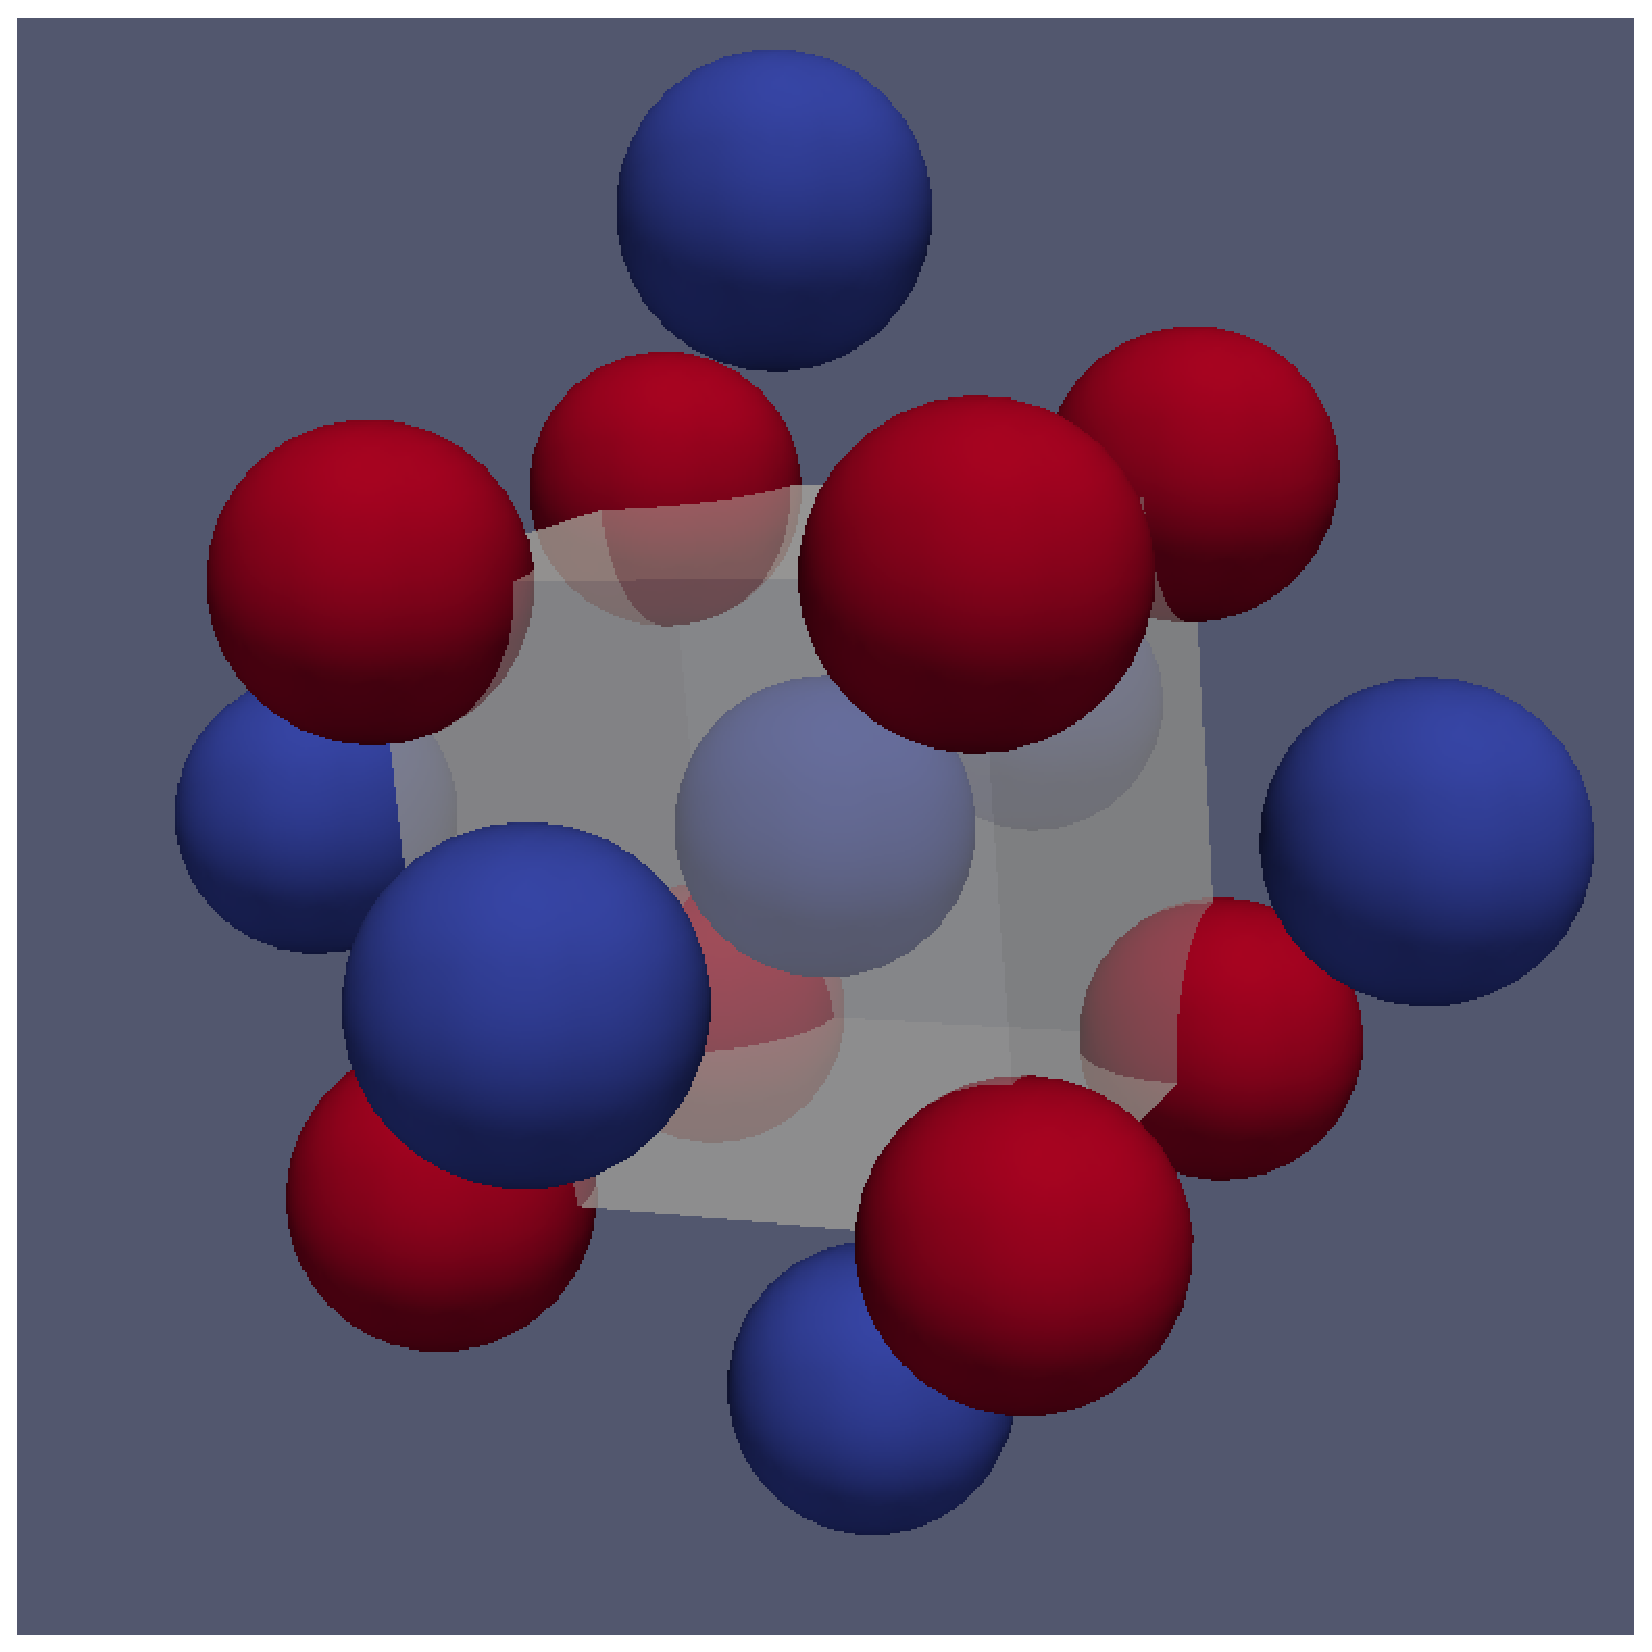
\includegraphics[width=0.27\textwidth]{bcc_15} & 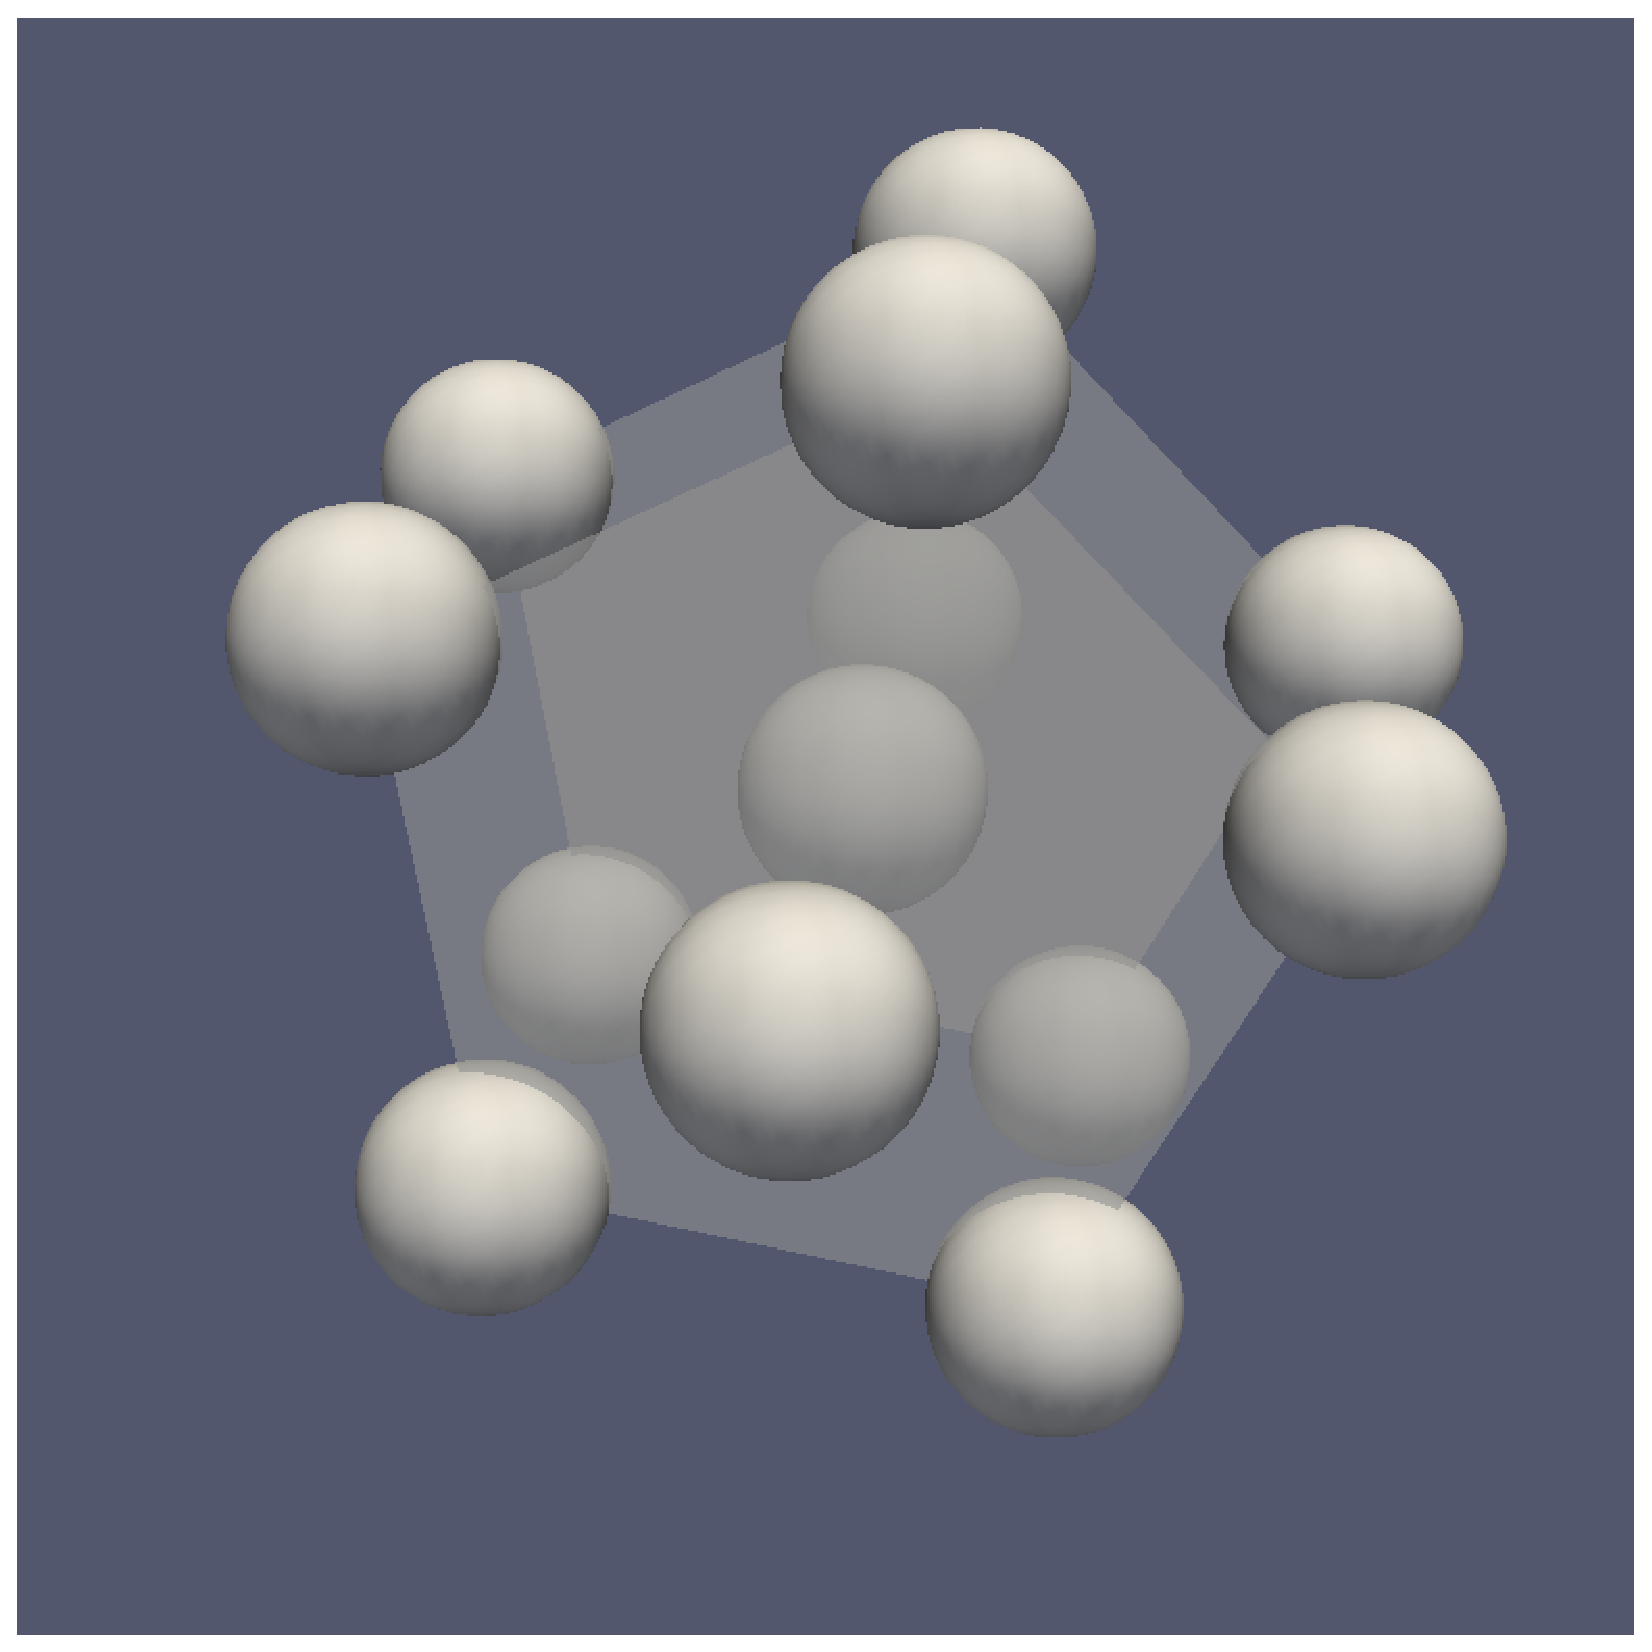
\includegraphics[width=0.27\textwidth]{dodec_13} \\ 
	BCC 9 & BCC 15 & Dodecadehron \\ 
	\end{tabular}}%
	\end{center}
	\only<all:2>{%
	\begin{itemize}
		\item The best ways to pack particles
		\item In hard spheres
		\begin{itemize}
			\item no potential energy
			\item ordering maximizes local vibrations
			\item vibrational entropy $\Leftrightarrow$ configurational entropy
			\item packing drives ordering
		\end{itemize}
	\end{itemize}
	
	\bigskip}%
\end{frame}

\begin{frame}[label=local_sym_sh]{Local symmetries and spherical harmonics}
	\begin{columns}
	\centering
	\column{0.25\textwidth}
	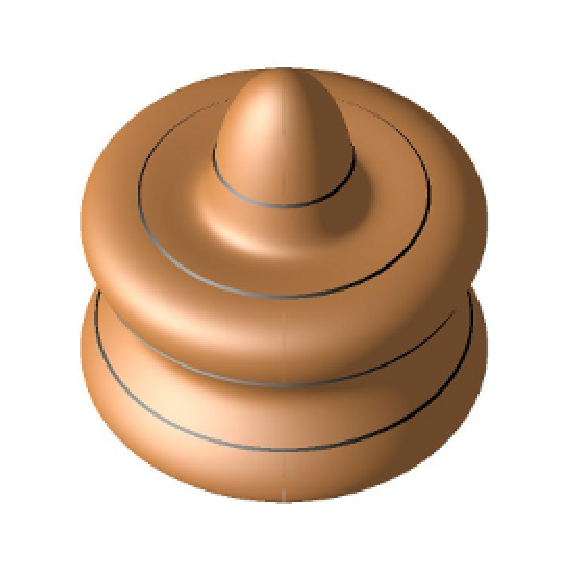
\includegraphics[width=\columnwidth]{sh6-0}\\
	\centering{$\ell=6, m=0$}
	\column{0.05\textwidth}
	$+$
	\column{0.25\textwidth}
	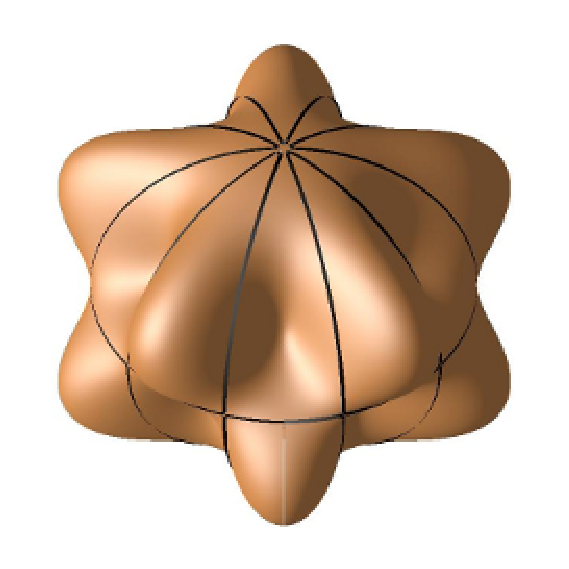
\includegraphics[width=\columnwidth]{sh6-5}\\
	\centering{$\ell=6, m=5$}
	\column{0.05\textwidth}
	$=$
	\column{0.3\textwidth}
	\centering{Icosahedron}\\
	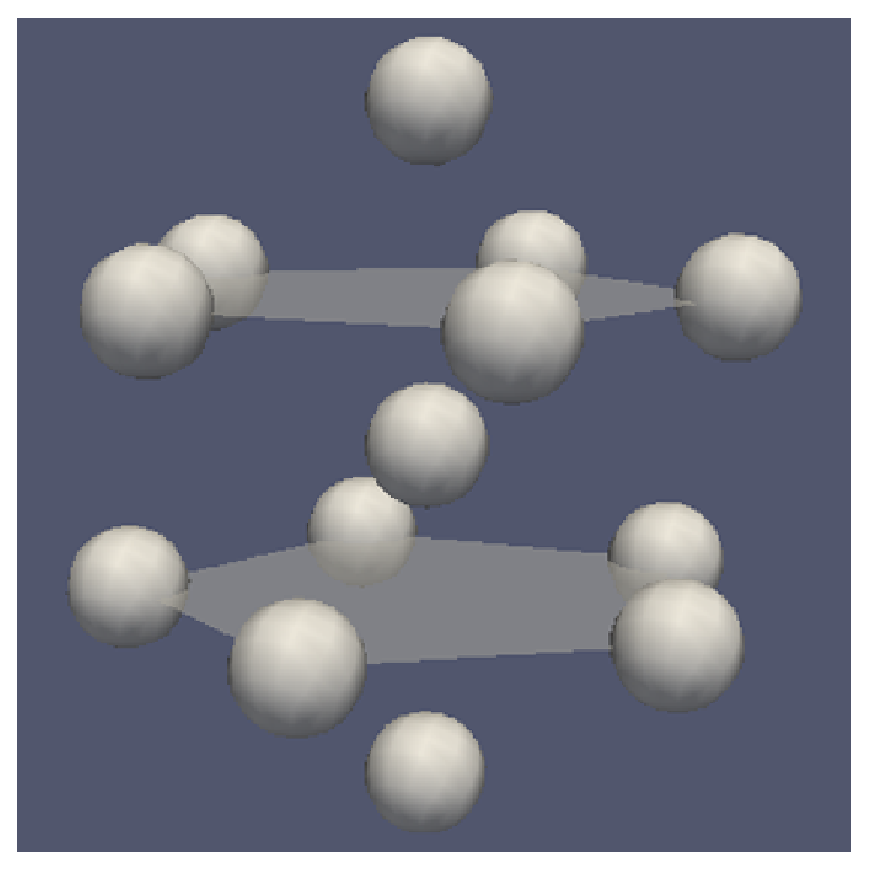
\includegraphics[width=\columnwidth]{ico_13}
	\end{columns}
	
	\begin{columns}
	\centering
	\column{0.25\textwidth}
	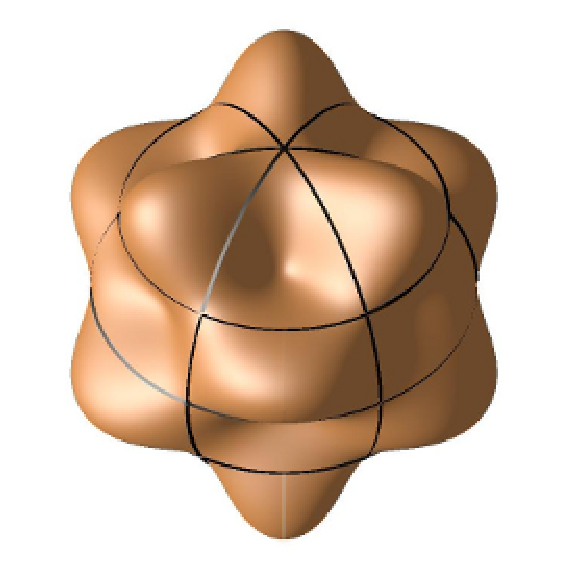
\includegraphics[width=\columnwidth]{sh6-3}\\
	\centering{$\ell=6, m=3$}
	\column{0.05\textwidth}
	$+$
	\column{0.25\textwidth}
	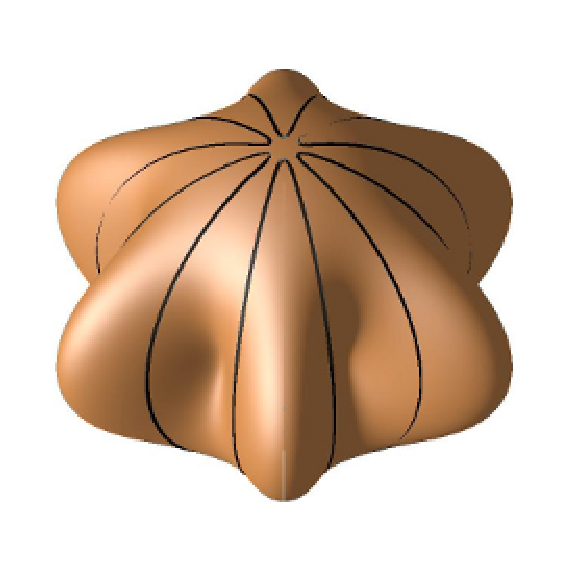
\includegraphics[width=\columnwidth]{sh6-6}\\
	\centering{$\ell=6, m=6$}
	\column{0.05\textwidth}
	$=$
	\column{0.3\textwidth}
	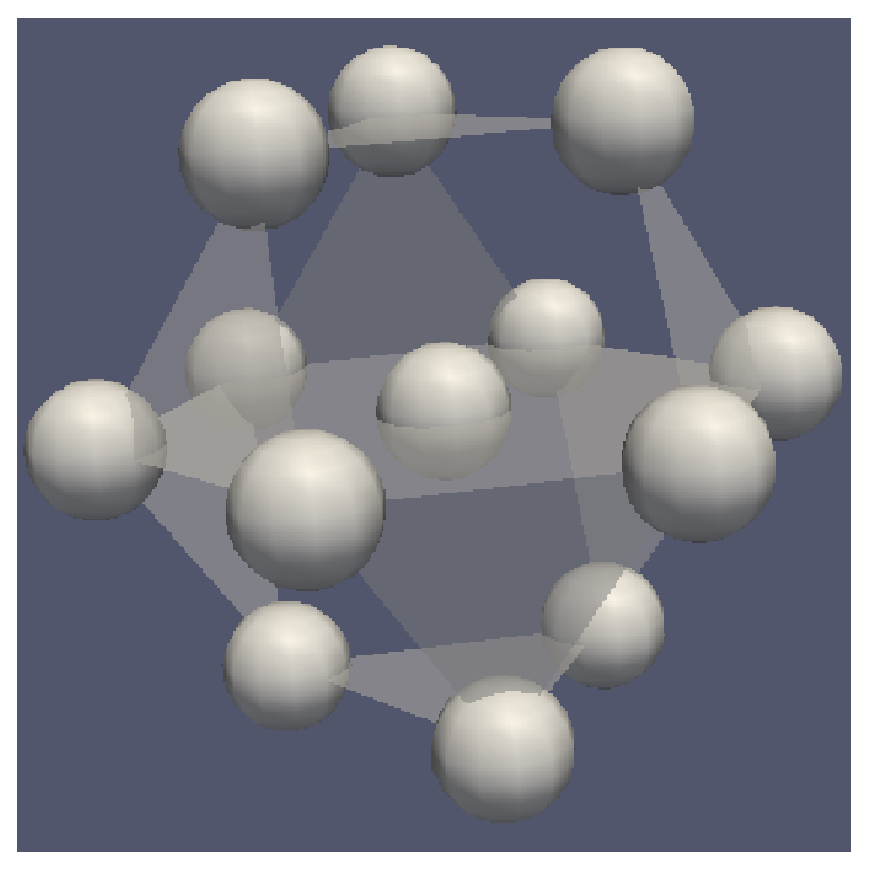
\includegraphics[width=\columnwidth]{fcc_13}\\
	\centering{FCC}
	\end{columns}
\end{frame}

\begin{frame}{Bond orientational order}
	\begin{columns}
	\column{0.5\textwidth}
	\includegraphics[width=\columnwidth]{lechner_Q4Q6}
	\column{0.5\textwidth}
	\begin{itemize}
		\item $Q_\ell$ is the strength of the $\ell$-fold symmetry
		\item Very good at telling apart
			\begin{itemize}
				\item aperiodic structures
				\item locally periodic
			\end{itemize}
		\item Differentiate between crystal structures
	\end{itemize}
	\end{columns}
	
	\bigskip
	\begin{footnotesize}
		\bibentry{steinhardt1983boo}
		\bibentry{lechner:114707}
	\end{footnotesize}
\end{frame}

\begin{frame}{Crystal-like bond order}
	\begin{textblock*}{0.6\textwidth}(10mm,92mm)
		\simplephasediagram{}
	\end{textblock*}
	\begin{columns}
	\column{0.65\textwidth}
	\resizebox{1.15\columnwidth}{!}{\input{Q4Q6quarter.pdf_tex}}
	\column{0.35\textwidth}
	\begin{itemize}
		\item Appear at $\phi_F$
		\item Develop at deep supercooling
		\item Not BCC
	\end{itemize}
	\end{columns}
\end{frame}

\begin{frame}{$\ldots$ is FCC-like}
	\begin{textblock*}{0.6\textwidth}(10mm,92mm)
		\simplephasediagram{}
	\end{textblock*}
	\begin{columns}
	\column{0.65\textwidth}
	\resizebox{1.15\columnwidth}{!}{\input{W4Q6quarter.pdf_tex}}
	\column{0.35\textwidth}
	\begin{itemize}
		\item $W_\ell$ indicates how the $\ell$-fold symmetry is "rotating"
		\item Uniform tail at shallow supercooling
		\item Clearly FCC at deep supercooling
		\item Not HCP
	\end{itemize}
	
	\bigskip
	\centering Ok to keep only $Q_6$ as \alert{crystal-like axis}
	\end{columns}
\end{frame}

\begin{frame}<all:1>[label=ico_axis]{Icosahedral axis}
	%\tikzstyle{background grid}=[draw, black!50,step=0.1\textwidth]
    \begin{tikzpicture}[xscale=38]
    	\draw[->, very thick] (-0.1697,0) -- (0.10,0) node[below left]{$w_6$};
    	\draw[thick] (-0.1697, 0.3em) -- (-0.1697, -0.3em) node[below]{$w_6^{ico}$}
    		(-0.0937, 0.3em) -- (-0.0937,-0.3em) node[below]{$w_6^{dodec}$}
    		(0, 0.3em) -- (0,-0.3em) node[below]{$0$};
    	\draw<all:2>[thick] (-0.15, 0.3em) -- (-0.15, -0.3em) node[below]{$w_6^*$};
    	\draw[dashed] (-0.1697, 0.3em) -- (-0.1697, 2em) node [inner sep=0pt,above right] (ico){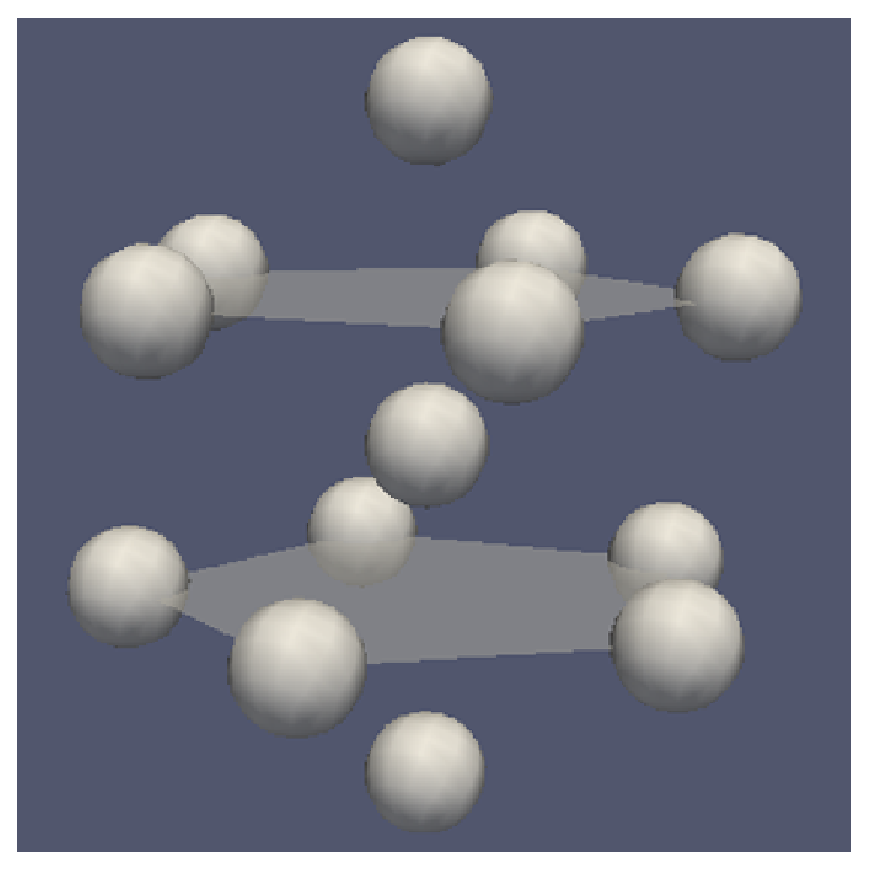
\includegraphics[width=0.22\textwidth]{ico_13}};
    	\node[below] at (ico.south) {Icosahedron};
    	\draw[dashed] (-0.0937, 0.3em) -- (-0.0937, 2em) node [inner sep=0pt,above right] (dodec){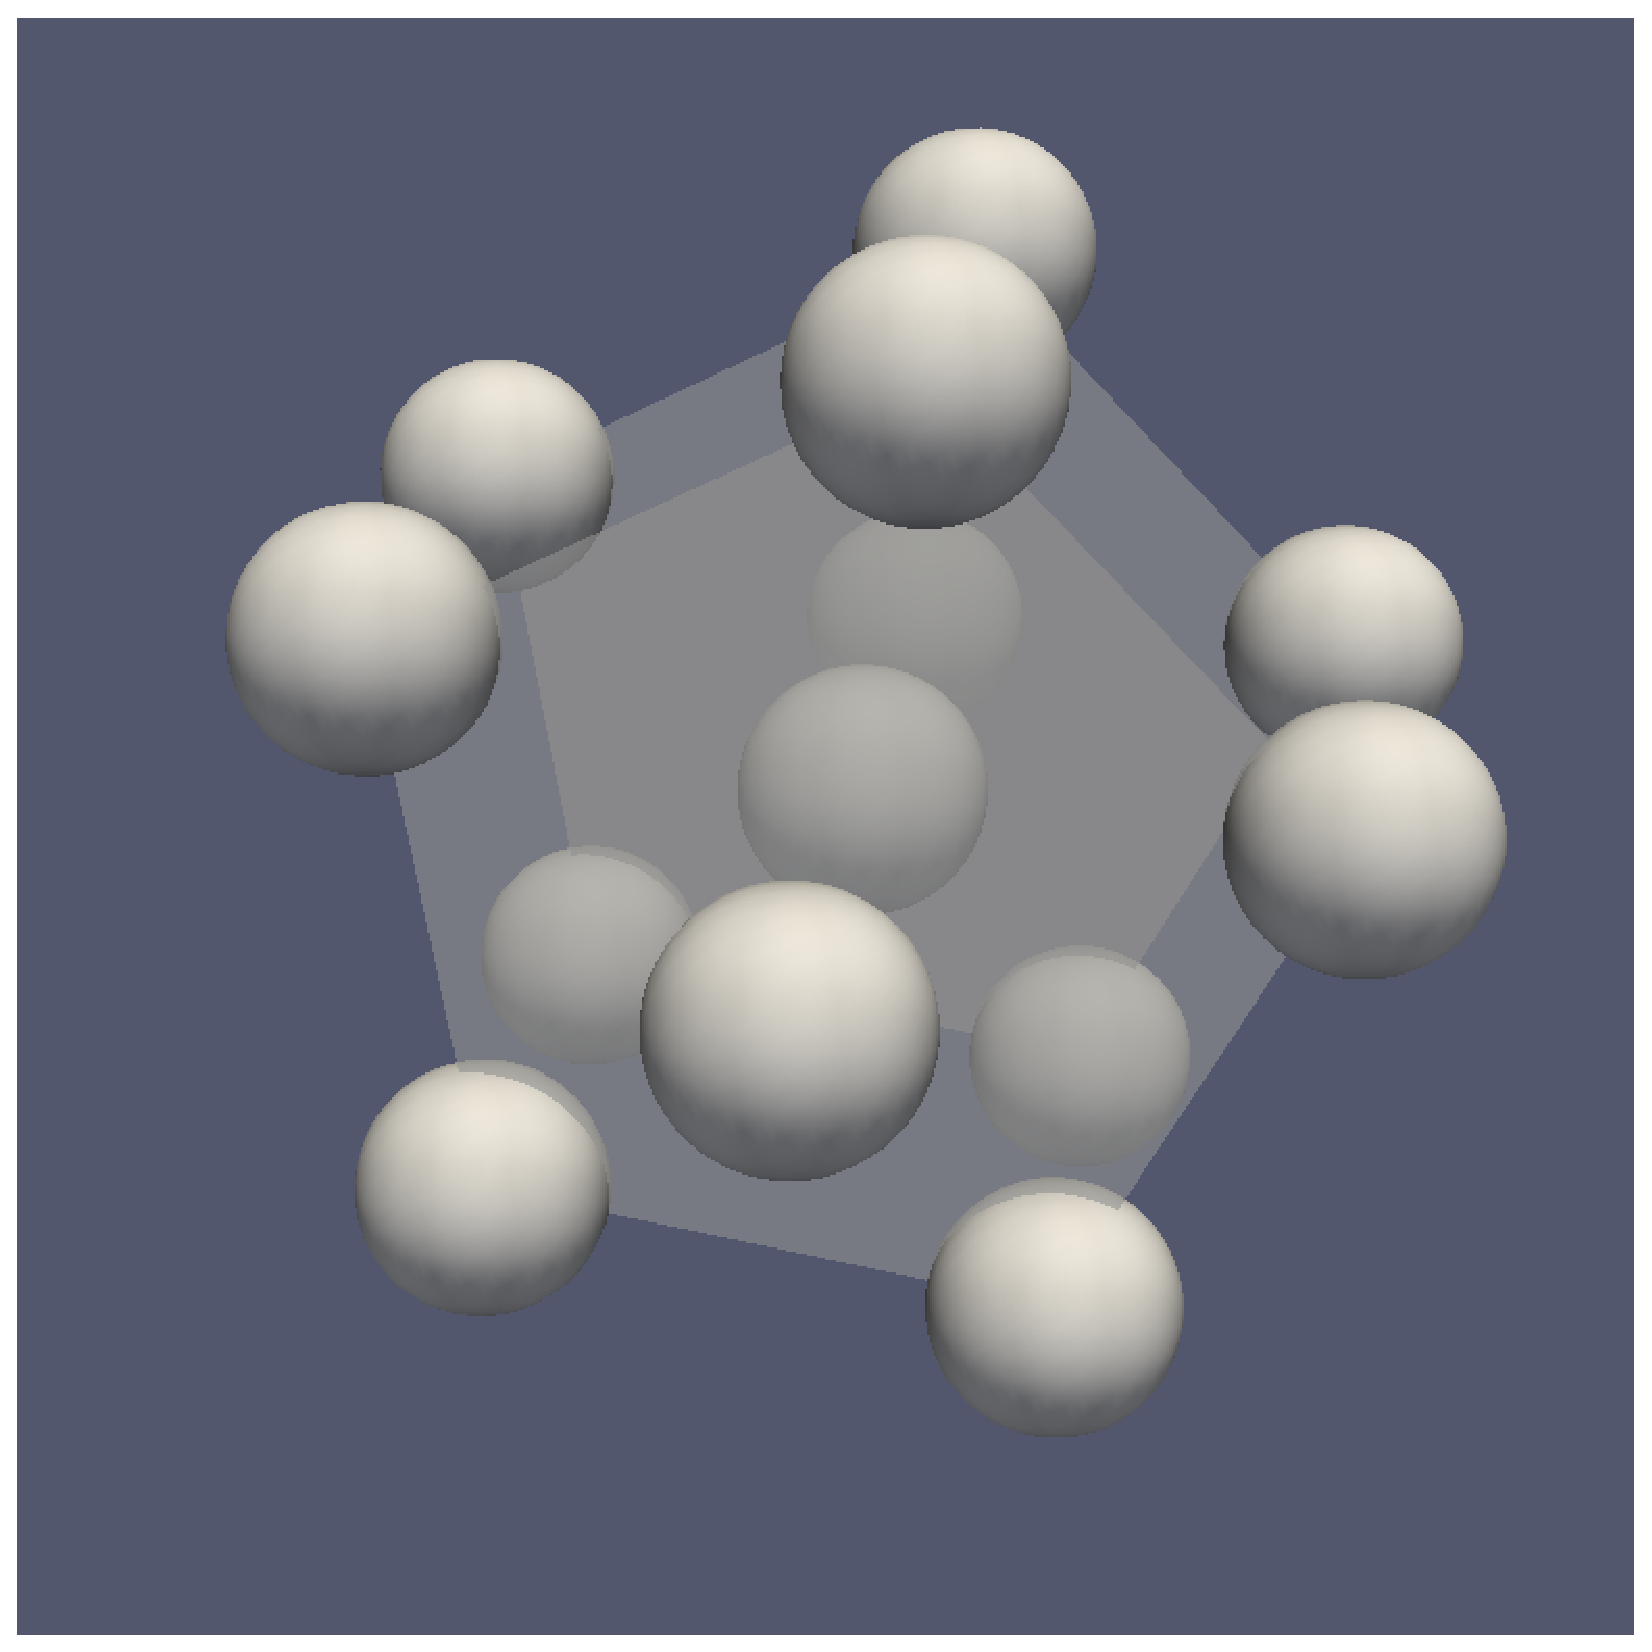
\includegraphics[width=0.22\textwidth]{dodec_13}};
    	\node[below] at (dodec.south) {Dodecahedron};
	\end{tikzpicture}
	
	\alt<all:1>{\begin{columns}
	\column{0.5\textwidth}
	$w_6^{ico}$ is the absolute minimum 
	\[ w_6^{ico}= -\frac{11}{\sqrt{4199}} \sim -0.1697 \]
	\column{0.5\textwidth}
	\begin{itemize}
		\item Icosahedra exist in attractive systems
		\item In hard spheres: only packing
		\item Not looked for except at $\phi>\phi_g$
	\end{itemize}
	\end{columns}}%
	{$w_6^* \simeq 0.15$ differentiate between
	\begin{itemize}
		\item perfect (stable) icosahedra
		\item imperfect (less stable) icosahedra
	\end{itemize}}
\end{frame}

\begin{frame}{Icosahedral order}
	\begin{textblock*}{0.6\textwidth}(10mm,92mm)
		\simplephasediagram{}
	\end{textblock*}
	\begin{columns}
	\column{0.65\textwidth}
	\resizebox{1.15\columnwidth}{!}{\input{w6Q6quarter.pdf_tex}}
	\column{0.35\textwidth}
	\begin{itemize}
		\item Already in the normal liquid
		\item Increases with supercooling
	\end{itemize}
	\end{columns}
\end{frame}

\begin{frame}<all:1->{Two types of orders in real space}
	\begin{textblock*}{0.6\textwidth}(10mm,92mm)
		\simplephasediagram{%
		\node<all:1> at (0.497,0) [xp marker, fill=green!50!black] {};
		\node<all:2> at (0.535,0) [xp marker, fill=green!50!black] {};
		\node<all:3> at (0.576,0) [xp marker, fill=green!50!black] {};
		}
	\end{textblock*}
	\begin{columns}[T]
	\column{0.6\textwidth}
	\only<all:1>{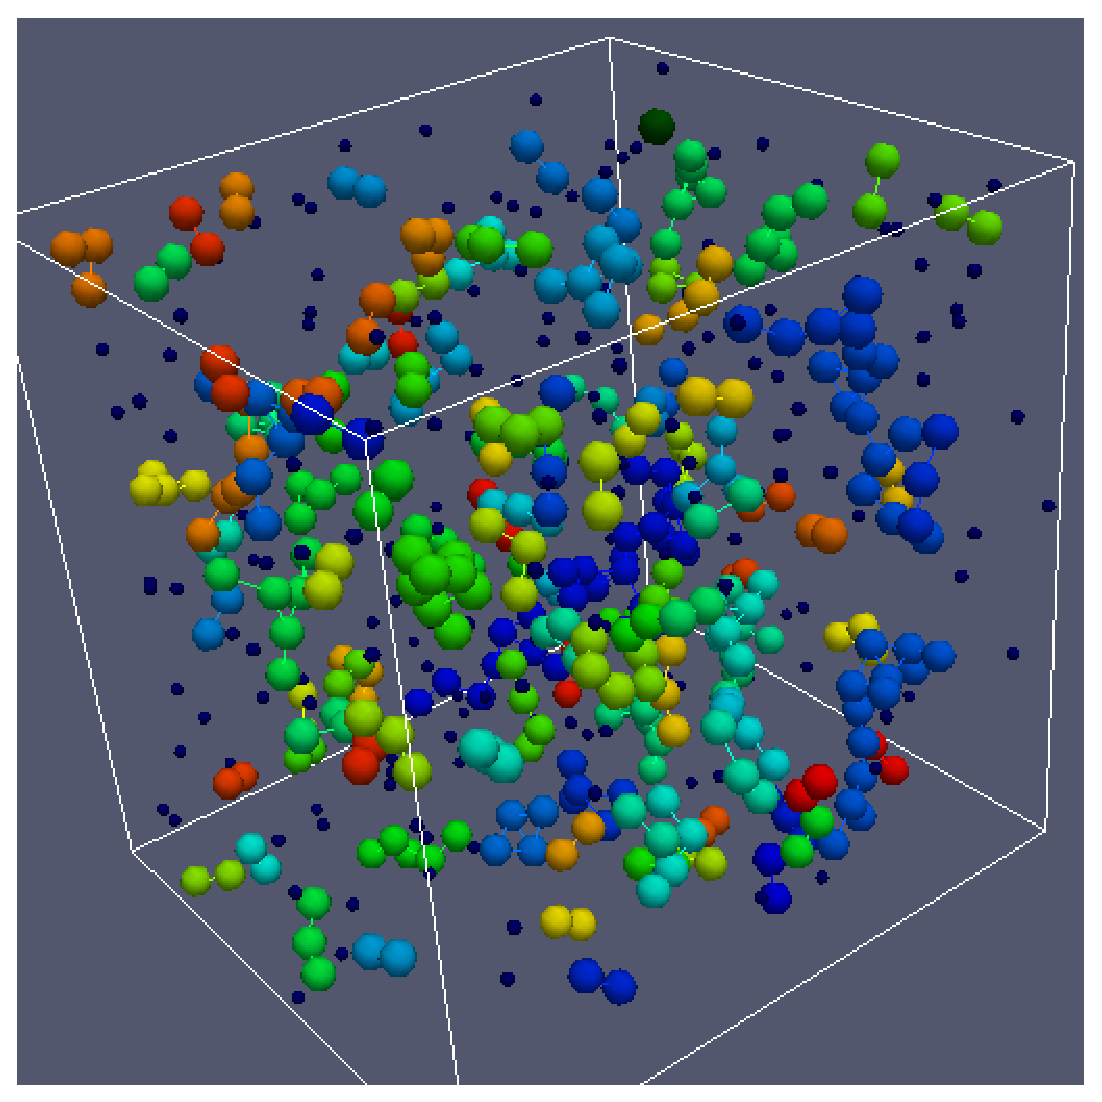
\includegraphics[width=\columnwidth]{mrco_alphabonds_3954}
	\[ \phi=0.497 \]}%
	\only<all:2>{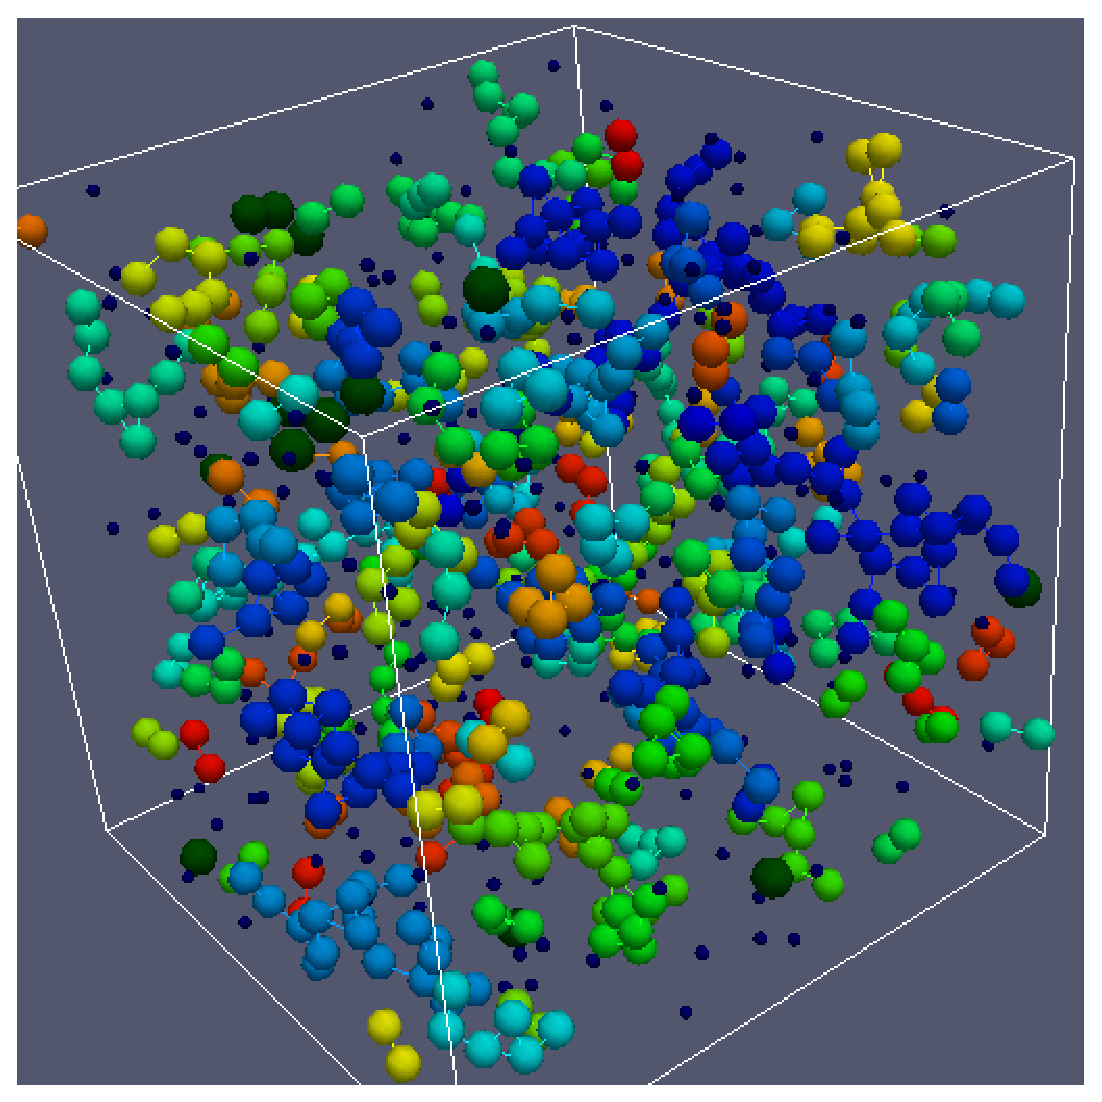
\includegraphics[width=\columnwidth]{mrco_alphabonds_4582}
	\[ \phi=0.535 \]}%
	\only<all:3>{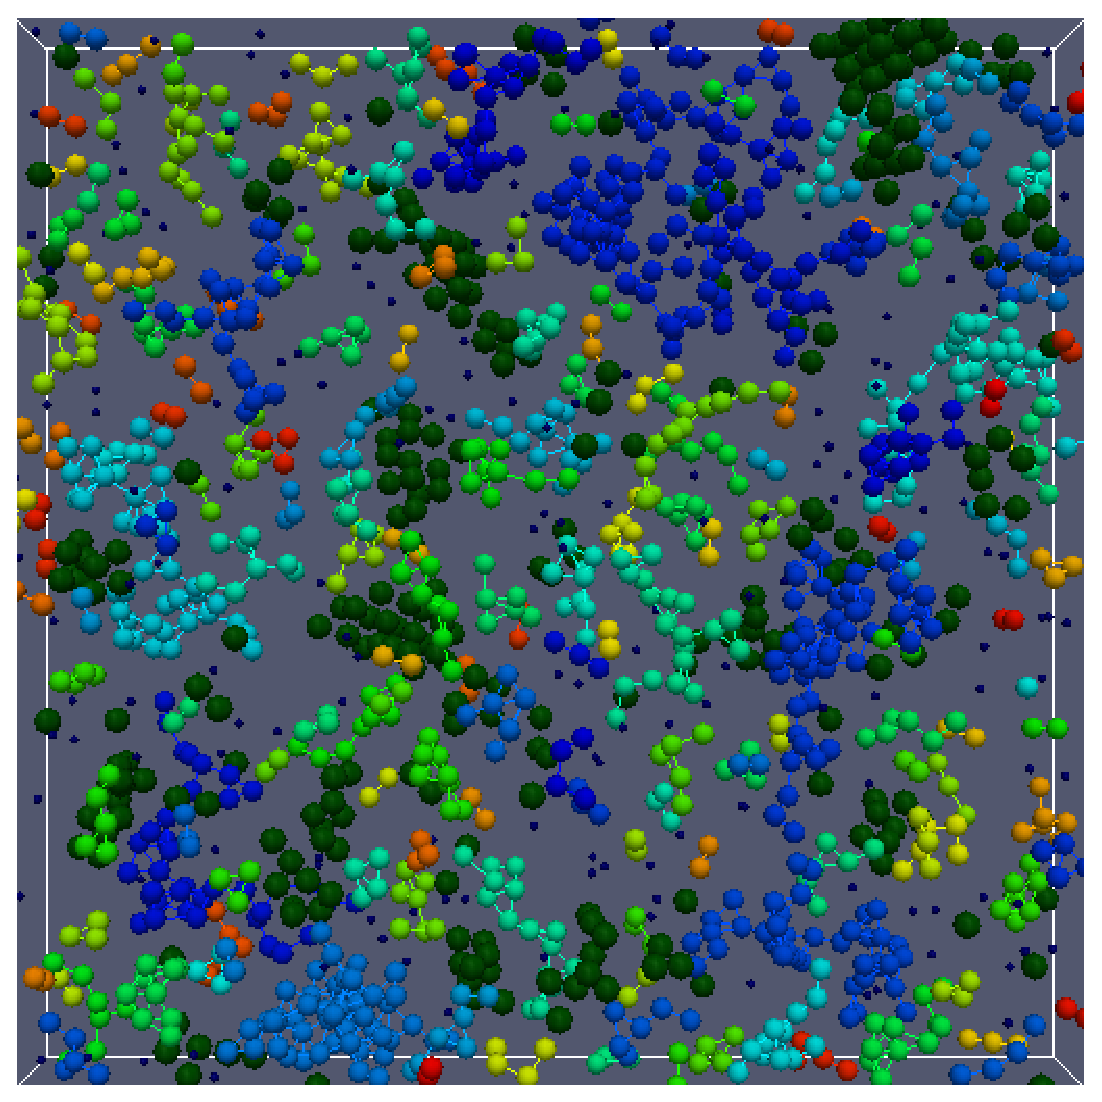
\includegraphics[width=\columnwidth]{mrco_alphabonds_go1}
	\[ \phi=0.576 \]}%
	\column{0.4\textwidth}
	\begin{block}{Central particle}
	\begin{itemize}
		\item Crystal-like \tikz\shade[ball color=green!33!black] (0,0) circle (0.5em);
		\item Icosahedra 
		\begin{itemize}
			\item isolated \tikz\shade[ball color=blue!50!black] (0,0) circle (0.3em);
			\item connected 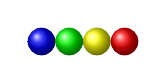
\begin{tikzpicture}
				\shade[ball color=blue] (0,0) circle (0.5em);
				\shade[ball color=green] +(1em,0) circle (0.5em);
				\shade[ball color=yellow] +(2em,0) circle (0.5em);
				\shade[ball color=red] +(3em,0) circle (0.5em);
				\end{tikzpicture}
		\end{itemize}
	\end{itemize}
	\end{block}
	\begin{itemize}
		\item Crystal-like \only<all:1>{order negligible}%
			\only<all:2>{order forms clusters}%
			\only<all:3> {compact clusters growing}%
		\item Icosahedral \only<all:1>{order forms strings}%
			\only<all:2>{order forms low dimensional clusters}%
			\only<all:3>{network percolates}%
	\end{itemize}
	\end{columns}
\end{frame}

\subsection{Characterisation}

\begin{frame}<1-| handout:1,3>{Local volume fraction along the \alt<all:1>{crystal-like}{icosahedral} axis}
	\begin{textblock*}{0.6\textwidth}(10mm,92mm)
		\simplephasediagram{}
	\end{textblock*}
	\begin{columns}
	\column{0.3\textwidth}
	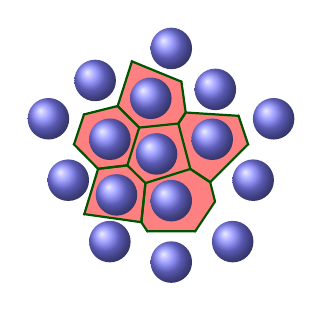
\begin{tikzpicture}[scale=0.13]
		\tikzset{particle/.style={circle, ball color=blue!50!white, inner sep=0, minimum size=1.5em}}
		\tikzset{vertice/.style={circle, ball color=red!50!white, inner sep=0}}
		\tikzset{edge/.style={thick, green!33!black}}
		\node [vertice] at (54.249, 39) (v2) {};
		\node [vertice] at (56.188, 41.909) (v3) {};
		\node [vertice] at (49.390, 43.713) (v5) {};
		\node [vertice] at (47.620, 45.446) (v6) {};
		\node [vertice] at (44.765, 45.106) (v7) {};
		\node [vertice] at (42.413, 47.493) (v8) {};
		\node [vertice] at (43.388, 50.418) (v9) {};
		\node [vertice] at (52.905, 53.618) (v10) {};
		\node [vertice] at (48.781, 49.134) (v11) {};
		\node [vertice] at (48.073, 55.602) (v12) {};
		\node [vertice] at (46.675, 51.240) (v13) {};
		\node [vertice] at (53.776, 45.093) (v14) {};
		\node [vertice] at (55.715, 43.8) (v15) {};
		\node [vertice] at (52.603, 49.531) (v16) {};
		\node [vertice] at (53.321, 50.608) (v17) {};
		\node [vertice] at (59.416, 47.5) (v18) {};
		\node [vertice] at (58.488, 50.283) (v19) {};
		\node [vertice] at (49.582, 39) (v20) {};
		\node [vertice] at (48.988, 39.891) (v21) {};
		\node [vertice] at (43.416, 40.682) (v23) {};
		\fill<all:1-2>[red!50!white] (v5.center) -- (v6.center) -- (v11.center) -- (v16.center) -- (v14.center) -- cycle;
		\fill<all:3>[red!50!white] (v2.center) -- (v3.center) -- (v15.center) -- (v18.center) -- (v19.center) -- (v17.center) -- (v10.center) -- (v12.center) -- (v13.center) -- (v9.center) -- (v8.center) -- (v7.center) -- (v23.center) -- (v21.center) -- (v20.center) -- cycle;
		\draw[edge] (v2.center) -- (v3.center) -- (v15.center) -- (v14.center) -- (v5.center) -- (v21.center) -- (v20.center) -- cycle;
		\draw[edge] (v5.center) -- (v6.center) -- (v7.center) -- (v23.center) -- (v21.center) -- cycle;
		\draw[edge] (v6.center) -- (v7.center) -- (v8.center) -- (v9.center) -- (v13.center) -- (v11.center) -- cycle;
		\draw[edge] (v11.center) -- (v16.center) -- (v17.center) -- (v10.center) -- (v12.center) -- (v13.center) -- cycle;
		\draw[edge] (v14.center) -- (v15.center) -- (v18.center) -- (v19.center) -- (v17.center) -- (v16.center) -- cycle;
		\node [particle] at (51.916, 56.871) (p1) {};
		\node [particle] at (44.480, 53.742) (p2) {};
		\node [particle] at (49.916, 52.000) (p3) {};
		\node [particle] at (56.222, 52.871) (p4) {};
		\node [particle] at (39.916, 50.000) (p5) {};
		\node [particle] at (45.916, 48.000) (p6) {};
		\node [particle] at (50.480, 46.564) (p7) {};
		\node [particle] at (55.916, 48.000) (p8) {};
		\node [particle] at (61.916, 50.000) (p9) {};
		\node [particle] at (41.854, 44.000) (p10) {};
		\node [particle] at (46.564, 42.564) (p11) {};
		\node [particle] at (51.916, 42.000) (p12) {};
		\node [particle] at (59.916, 44.000) (p13) {};
		\node [particle] at (45.916, 38.000) (p15) {};
		\node [particle] at (51.916, 36.000) (p16) {};
		\node [particle] at (57.916, 38.000) (p17) {};
	\end{tikzpicture}
	\column{0.7\textwidth}
	\resizebox{\columnwidth}{!}{%
		\only<all:1>{% GNUPLOT: LaTeX picture with Postscript
\begingroup
  \makeatletter
  \providecommand\color[2][]{%
    \GenericError{(gnuplot) \space\space\space\@spaces}{%
      Package color not loaded in conjunction with
      terminal option `colourtext'%
    }{See the gnuplot documentation for explanation.%
    }{Either use 'blacktext' in gnuplot or load the package
      color.sty in LaTeX.}%
    \renewcommand\color[2][]{}%
  }%
  \providecommand\includegraphics[2][]{%
    \GenericError{(gnuplot) \space\space\space\@spaces}{%
      Package graphicx or graphics not loaded%
    }{See the gnuplot documentation for explanation.%
    }{The gnuplot epslatex terminal needs graphicx.sty or graphics.sty.}%
    \renewcommand\includegraphics[2][]{}%
  }%
  \providecommand\rotatebox[2]{#2}%
  \@ifundefined{ifGPcolor}{%
    \newif\ifGPcolor
    \GPcolortrue
  }{}%
  \@ifundefined{ifGPblacktext}{%
    \newif\ifGPblacktext
    \GPblacktexttrue
  }{}%
  % define a \g@addto@macro without @ in the name:
  \let\gplgaddtomacro\g@addto@macro
  % define empty templates for all commands taking text:
  \gdef\gplbacktext{}%
  \gdef\gplfronttext{}%
  \makeatother
  \ifGPblacktext
    % no textcolor at all
    \def\colorrgb#1{}%
    \def\colorgray#1{}%
  \else
    % gray or color?
    \ifGPcolor
      \def\colorrgb#1{\color[rgb]{#1}}%
      \def\colorgray#1{\color[gray]{#1}}%
      \expandafter\def\csname LTw\endcsname{\color{white}}%
      \expandafter\def\csname LTb\endcsname{\color{black}}%
      \expandafter\def\csname LTa\endcsname{\color{black}}%
      \expandafter\def\csname LT0\endcsname{\color[rgb]{1,0,0}}%
      \expandafter\def\csname LT1\endcsname{\color[rgb]{0,1,0}}%
      \expandafter\def\csname LT2\endcsname{\color[rgb]{0,0,1}}%
      \expandafter\def\csname LT3\endcsname{\color[rgb]{1,0,1}}%
      \expandafter\def\csname LT4\endcsname{\color[rgb]{0,1,1}}%
      \expandafter\def\csname LT5\endcsname{\color[rgb]{1,1,0}}%
      \expandafter\def\csname LT6\endcsname{\color[rgb]{0,0,0}}%
      \expandafter\def\csname LT7\endcsname{\color[rgb]{1,0.3,0}}%
      \expandafter\def\csname LT8\endcsname{\color[rgb]{0.5,0.5,0.5}}%
    \else
      % gray
      \def\colorrgb#1{\color{black}}%
      \def\colorgray#1{\color[gray]{#1}}%
      \expandafter\def\csname LTw\endcsname{\color{white}}%
      \expandafter\def\csname LTb\endcsname{\color{black}}%
      \expandafter\def\csname LTa\endcsname{\color{black}}%
      \expandafter\def\csname LT0\endcsname{\color{black}}%
      \expandafter\def\csname LT1\endcsname{\color{black}}%
      \expandafter\def\csname LT2\endcsname{\color{black}}%
      \expandafter\def\csname LT3\endcsname{\color{black}}%
      \expandafter\def\csname LT4\endcsname{\color{black}}%
      \expandafter\def\csname LT5\endcsname{\color{black}}%
      \expandafter\def\csname LT6\endcsname{\color{black}}%
      \expandafter\def\csname LT7\endcsname{\color{black}}%
      \expandafter\def\csname LT8\endcsname{\color{black}}%
    \fi
  \fi
  \setlength{\unitlength}{0.0500bp}%
  \begin{picture}(7200.00,5040.00)%
    \gplgaddtomacro\gplbacktext{%
      \csname LTb\endcsname%
      \put(1056,2520){\makebox(0,0)[r]{\strut{}$0.4$}}%
      \put(1056,3165){\makebox(0,0)[r]{\strut{}$0.5$}}%
      \put(1056,3809){\makebox(0,0)[r]{\strut{}$0.6$}}%
      \put(1056,4454){\makebox(0,0)[r]{\strut{}$0.7$}}%
      \put(1188,2300){\makebox(0,0){\strut{}}}%
      \put(1931,2300){\makebox(0,0){\strut{}}}%
      \put(2674,2300){\makebox(0,0){\strut{}}}%
      \put(3417,2300){\makebox(0,0){\strut{}}}%
      \put(4160,2300){\makebox(0,0){\strut{}}}%
      \put(4903,2300){\makebox(0,0){\strut{}}}%
      \put(5646,2300){\makebox(0,0){\strut{}}}%
      \put(6389,2300){\makebox(0,0){\strut{}}}%
      \put(418,3648){\rotatebox{-270}{\makebox(0,0){\strut{}$<\tilde{\phi}_{local}>$}}}%
      \put(6979,3648){\rotatebox{-270}{\makebox(0,0){\strut{}}}}%
      \put(3974,4666){\makebox(0,0){\strut{}}}%
      \put(3974,4665){\makebox(0,0){\strut{}}}%
      \put(264,2410){\makebox(0,0)[l]{\strut{}}}%
    }%
    \gplgaddtomacro\gplfronttext{%
      \put(5424,4603){\makebox(0,0){\strut{}Experiments}}%
      \csname LTb\endcsname%
      \put(5805,3569){\makebox(0,0)[r]{\strut{}$\phi=0.497$}}%
      \csname LTb\endcsname%
      \put(5805,3833){\makebox(0,0)[r]{\strut{}$\phi=0.535$}}%
      \csname LTb\endcsname%
      \put(5805,4097){\makebox(0,0)[r]{\strut{}$\phi=0.555$}}%
      \csname LTb\endcsname%
      \put(5805,4361){\makebox(0,0)[r]{\strut{}$\phi=0.576$}}%
    }%
    \gplgaddtomacro\gplbacktext{%
      \csname LTb\endcsname%
      \put(1056,704){\makebox(0,0)[r]{\strut{}$0.4$}}%
      \put(1056,1223){\makebox(0,0)[r]{\strut{}$0.5$}}%
      \put(1056,1741){\makebox(0,0)[r]{\strut{}$0.6$}}%
      \put(1056,2260){\makebox(0,0)[r]{\strut{}$0.7$}}%
      \put(1188,484){\makebox(0,0){\strut{}$0$}}%
      \put(1931,484){\makebox(0,0){\strut{}$0.1$}}%
      \put(2674,484){\makebox(0,0){\strut{}$0.2$}}%
      \put(3417,484){\makebox(0,0){\strut{}$0.3$}}%
      \put(4160,484){\makebox(0,0){\strut{}$0.4$}}%
      \put(4903,484){\makebox(0,0){\strut{}$0.5$}}%
      \put(5646,484){\makebox(0,0){\strut{}$0.6$}}%
      \put(6389,484){\makebox(0,0){\strut{}$0.7$}}%
      \put(418,1611){\rotatebox{-270}{\makebox(0,0){\strut{}$<\phi_{local}>$}}}%
      \put(6979,1611){\rotatebox{-270}{\makebox(0,0){\strut{}}}}%
      \put(3974,154){\makebox(0,0){\strut{}$Q_6$}}%
      \put(3974,2409){\makebox(0,0){\strut{}}}%
      \put(3974,2408){\makebox(0,0){\strut{}}}%
      \put(264,110){\makebox(0,0)[l]{\strut{}}}%
    }%
    \gplgaddtomacro\gplfronttext{%
      \put(5358,2346){\makebox(0,0){\strut{}Simulations}}%
      \csname LTb\endcsname%
      \put(5805,1048){\makebox(0,0)[r]{\strut{}$\phi=0.487$ }}%
      \csname LTb\endcsname%
      \put(5805,1312){\makebox(0,0)[r]{\strut{}$\phi=0.507$ }}%
      \csname LTb\endcsname%
      \put(5805,1576){\makebox(0,0)[r]{\strut{}$\phi=0.528$ }}%
      \csname LTb\endcsname%
      \put(5805,1840){\makebox(0,0)[r]{\strut{}$\phi=0.548$ }}%
      \csname LTb\endcsname%
      \put(5805,2104){\makebox(0,0)[r]{\strut{}$\phi=0.568$ }}%
    }%
    \gplbacktext
    \put(0,0){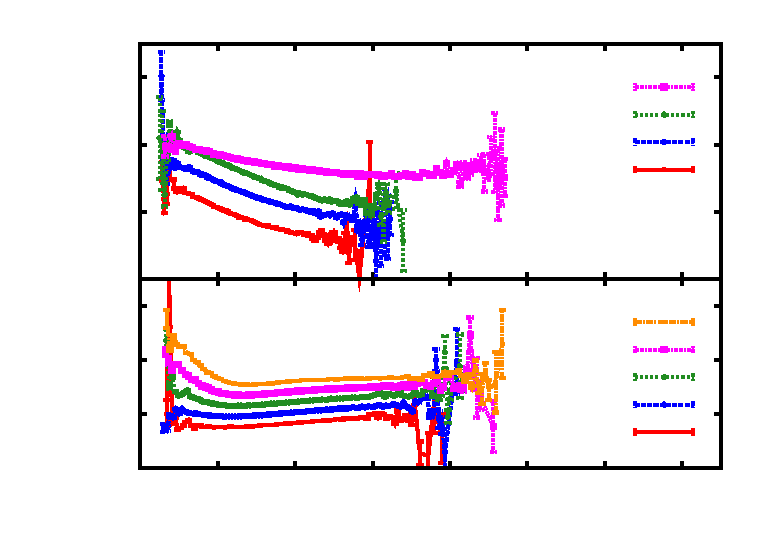
\includegraphics{phi_Q6_xpsim}}%
    \gplfronttext
  \end{picture}%
\endgroup
}%
		\only<all:2>{\input{phi_w6_xpsim_local}}%
		\only<all:3>{% GNUPLOT: LaTeX picture with Postscript
\begingroup
  \makeatletter
  \providecommand\color[2][]{%
    \GenericError{(gnuplot) \space\space\space\@spaces}{%
      Package color not loaded in conjunction with
      terminal option `colourtext'%
    }{See the gnuplot documentation for explanation.%
    }{Either use 'blacktext' in gnuplot or load the package
      color.sty in LaTeX.}%
    \renewcommand\color[2][]{}%
  }%
  \providecommand\includegraphics[2][]{%
    \GenericError{(gnuplot) \space\space\space\@spaces}{%
      Package graphicx or graphics not loaded%
    }{See the gnuplot documentation for explanation.%
    }{The gnuplot epslatex terminal needs graphicx.sty or graphics.sty.}%
    \renewcommand\includegraphics[2][]{}%
  }%
  \providecommand\rotatebox[2]{#2}%
  \@ifundefined{ifGPcolor}{%
    \newif\ifGPcolor
    \GPcolortrue
  }{}%
  \@ifundefined{ifGPblacktext}{%
    \newif\ifGPblacktext
    \GPblacktexttrue
  }{}%
  % define a \g@addto@macro without @ in the name:
  \let\gplgaddtomacro\g@addto@macro
  % define empty templates for all commands taking text:
  \gdef\gplbacktext{}%
  \gdef\gplfronttext{}%
  \makeatother
  \ifGPblacktext
    % no textcolor at all
    \def\colorrgb#1{}%
    \def\colorgray#1{}%
  \else
    % gray or color?
    \ifGPcolor
      \def\colorrgb#1{\color[rgb]{#1}}%
      \def\colorgray#1{\color[gray]{#1}}%
      \expandafter\def\csname LTw\endcsname{\color{white}}%
      \expandafter\def\csname LTb\endcsname{\color{black}}%
      \expandafter\def\csname LTa\endcsname{\color{black}}%
      \expandafter\def\csname LT0\endcsname{\color[rgb]{1,0,0}}%
      \expandafter\def\csname LT1\endcsname{\color[rgb]{0,1,0}}%
      \expandafter\def\csname LT2\endcsname{\color[rgb]{0,0,1}}%
      \expandafter\def\csname LT3\endcsname{\color[rgb]{1,0,1}}%
      \expandafter\def\csname LT4\endcsname{\color[rgb]{0,1,1}}%
      \expandafter\def\csname LT5\endcsname{\color[rgb]{1,1,0}}%
      \expandafter\def\csname LT6\endcsname{\color[rgb]{0,0,0}}%
      \expandafter\def\csname LT7\endcsname{\color[rgb]{1,0.3,0}}%
      \expandafter\def\csname LT8\endcsname{\color[rgb]{0.5,0.5,0.5}}%
    \else
      % gray
      \def\colorrgb#1{\color{black}}%
      \def\colorgray#1{\color[gray]{#1}}%
      \expandafter\def\csname LTw\endcsname{\color{white}}%
      \expandafter\def\csname LTb\endcsname{\color{black}}%
      \expandafter\def\csname LTa\endcsname{\color{black}}%
      \expandafter\def\csname LT0\endcsname{\color{black}}%
      \expandafter\def\csname LT1\endcsname{\color{black}}%
      \expandafter\def\csname LT2\endcsname{\color{black}}%
      \expandafter\def\csname LT3\endcsname{\color{black}}%
      \expandafter\def\csname LT4\endcsname{\color{black}}%
      \expandafter\def\csname LT5\endcsname{\color{black}}%
      \expandafter\def\csname LT6\endcsname{\color{black}}%
      \expandafter\def\csname LT7\endcsname{\color{black}}%
      \expandafter\def\csname LT8\endcsname{\color{black}}%
    \fi
  \fi
  \setlength{\unitlength}{0.0500bp}%
  \begin{picture}(7200.00,5040.00)%
    \gplgaddtomacro\gplbacktext{%
      \csname LTb\endcsname%
      \put(1056,2520){\makebox(0,0)[r]{\strut{}$0.4$}}%
      \put(1056,3165){\makebox(0,0)[r]{\strut{}$0.5$}}%
      \put(1056,3809){\makebox(0,0)[r]{\strut{}$0.6$}}%
      \put(1056,4454){\makebox(0,0)[r]{\strut{}$0.7$}}%
      \put(1369,2300){\makebox(0,0){\strut{}}}%
      \put(1791,2300){\makebox(0,0){\strut{}}}%
      \put(2394,2300){\makebox(0,0){\strut{}}}%
      \put(2997,2300){\makebox(0,0){\strut{}}}%
      \put(418,3648){\rotatebox{-270}{\makebox(0,0){\strut{}$<\tilde{\phi}_{local}>$}}}%
      \put(3819,3648){\rotatebox{-270}{\makebox(0,0){\strut{}}}}%
      \put(2394,4666){\makebox(0,0){\strut{}}}%
      \put(2394,4665){\makebox(0,0){\strut{}}}%
      \put(264,2190){\makebox(0,0)[l]{\strut{}}}%
    }%
    \gplgaddtomacro\gplfronttext{%
      \put(2557,4537){\makebox(0,0){\strut{}Experiments}}%
    }%
    \gplgaddtomacro\gplbacktext{%
      \csname LTb\endcsname%
      \put(3468,2520){\makebox(0,0)[r]{\strut{}}}%
      \put(3468,3165){\makebox(0,0)[r]{\strut{}}}%
      \put(3468,3809){\makebox(0,0)[r]{\strut{}}}%
      \put(3468,4454){\makebox(0,0)[r]{\strut{}}}%
      \put(3781,2300){\makebox(0,0){\strut{}}}%
      \put(4203,2300){\makebox(0,0){\strut{}}}%
      \put(4806,2300){\makebox(0,0){\strut{}}}%
      \put(5409,2300){\makebox(0,0){\strut{}}}%
      \put(6231,3648){\rotatebox{-270}{\makebox(0,0){\strut{}$<\tilde{\phi}_{ngb}>$}}}%
      \put(4806,4666){\makebox(0,0){\strut{}}}%
      \put(4806,4665){\makebox(0,0){\strut{}}}%
      \put(3336,2190){\makebox(0,0)[l]{\strut{}}}%
    }%
    \gplgaddtomacro\gplfronttext{%
      \csname LTb\endcsname%
      \put(4669,3877){\makebox(0,0)[r]{\strut{}$\phi=0.497$}}%
      \csname LTb\endcsname%
      \put(4669,4097){\makebox(0,0)[r]{\strut{}$\phi=0.535$}}%
      \csname LTb\endcsname%
      \put(4669,4317){\makebox(0,0)[r]{\strut{}$\phi=0.555$}}%
      \csname LTb\endcsname%
      \put(4669,4537){\makebox(0,0)[r]{\strut{}$\phi=0.576$}}%
    }%
    \gplgaddtomacro\gplbacktext{%
      \csname LTb\endcsname%
      \put(1056,704){\makebox(0,0)[r]{\strut{}$0.4$}}%
      \put(1056,1223){\makebox(0,0)[r]{\strut{}$0.5$}}%
      \put(1056,1741){\makebox(0,0)[r]{\strut{}$0.6$}}%
      \put(1056,2260){\makebox(0,0)[r]{\strut{}$0.7$}}%
      \put(1369,484){\makebox(0,0){\strut{}$-0.17$}}%
      \put(1791,484){\makebox(0,0){\strut{}$-0.1$}}%
      \put(2394,484){\makebox(0,0){\strut{}$0$}}%
      \put(2997,484){\makebox(0,0){\strut{}$0.1$}}%
      \put(418,1611){\rotatebox{90}{\makebox(0,0){\strut{}$<\phi_{local}>$}}}%
      \put(2394,154){\makebox(0,0){\strut{}$w_6$}}%
      \put(2394,2409){\makebox(0,0){\strut{}}}%
      \put(2394,2408){\makebox(0,0){\strut{}}}%
      \put(264,110){\makebox(0,0)[l]{\strut{}}}%
    }%
    \gplgaddtomacro\gplfronttext{%
      \put(2161,2305){\makebox(0,0){\strut{}Simulations}}%
      \csname LTb\endcsname%
      \put(2740,1865){\makebox(0,0)[r]{\strut{}$\phi=0.548$ }}%
      \csname LTb\endcsname%
      \put(2740,2085){\makebox(0,0)[r]{\strut{}$\phi=0.568$ }}%
    }%
    \gplgaddtomacro\gplbacktext{%
      \csname LTb\endcsname%
      \put(3468,704){\makebox(0,0)[r]{\strut{}}}%
      \put(3468,1223){\makebox(0,0)[r]{\strut{}}}%
      \put(3468,1741){\makebox(0,0)[r]{\strut{}}}%
      \put(3468,2260){\makebox(0,0)[r]{\strut{}}}%
      \put(3781,484){\makebox(0,0){\strut{}$-0.17$}}%
      \put(4203,484){\makebox(0,0){\strut{}$-0.1$}}%
      \put(4806,484){\makebox(0,0){\strut{}$0$}}%
      \put(5409,484){\makebox(0,0){\strut{}$0.1$}}%
      \put(6231,1611){\rotatebox{90}{\makebox(0,0){\strut{}$<\phi_{ngb}>$}}}%
      \put(4806,154){\makebox(0,0){\strut{}$w_6$}}%
      \put(4806,2409){\makebox(0,0){\strut{}}}%
      \put(4806,2408){\makebox(0,0){\strut{}}}%
      \put(3336,110){\makebox(0,0)[l]{\strut{}}}%
    }%
    \gplgaddtomacro\gplfronttext{%
      \csname LTb\endcsname%
      \put(4669,1865){\makebox(0,0)[r]{\strut{}$\phi=0.487$ }}%
      \csname LTb\endcsname%
      \put(4669,2085){\makebox(0,0)[r]{\strut{}$\phi=0.507$ }}%
      \csname LTb\endcsname%
      \put(4669,2305){\makebox(0,0)[r]{\strut{}$\phi=0.528$ }}%
    }%
    \gplbacktext
    \put(0,0){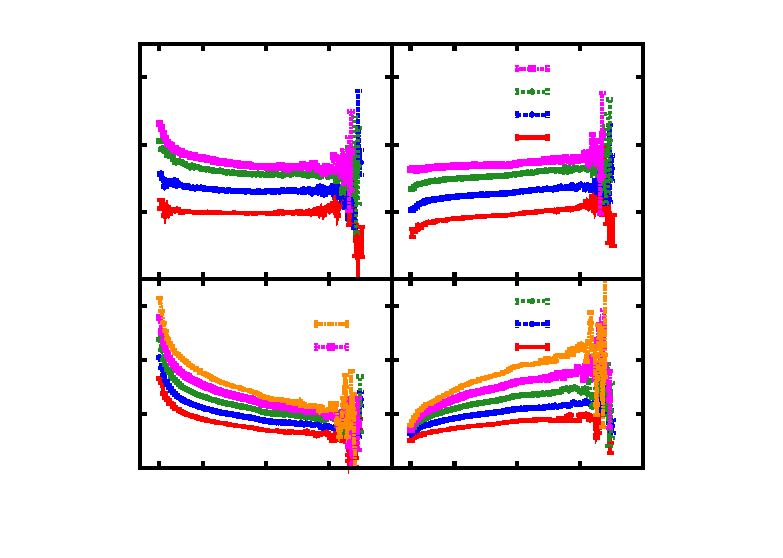
\includegraphics{phi_w6_xpsim_total}}%
    \gplfronttext
  \end{picture}%
\endgroup
}%
	}
	\end{columns}
	\alt<all:1>{%
	\begin{itemize}
		\item Crystallisation is a first order transition
		\item No steep change in density upon ordering
		\item Crystal-like bond ordered regions $\neq$ crystal
	\end{itemize}
	}{%
	\begin{itemize}
		\item Icosahedron's central particle has less free volume
		\item<3> Neighbours have more free volume $\Rightarrow$ stabilised
		\item<3> Much more stable below $w_6^* \simeq -0.15$
	\end{itemize}
	}%
\end{frame}

\againframe<all:2>{ico_axis}

\begin{frame}<all:1->{Perfect/imperfect icosahedra}
	\begin{textblock*}{0.6\textwidth}(10mm,92mm)
		\simplephasediagram{%
		\node<all:1> at (0.497,0) [xp marker, fill=green!50!black] {};
		\node<all:2> at (0.535,0) [xp marker, fill=green!50!black] {};
		\node<all:3> at (0.576,0) [xp marker, fill=green!50!black] {};
		}
	\end{textblock*}
	\begin{columns}[T]
	\column{0.6\textwidth}
	\only<all:1>{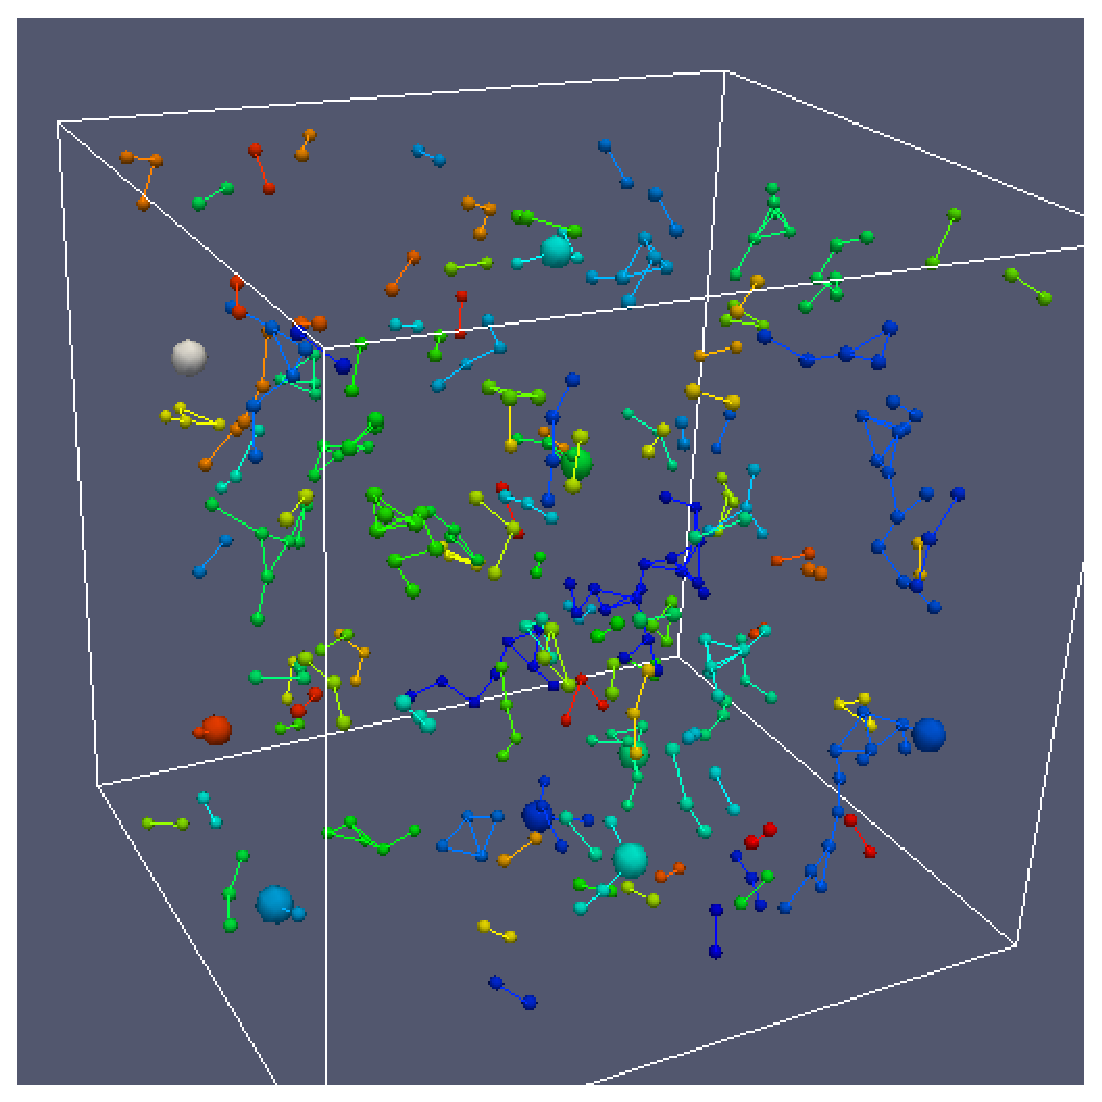
\includegraphics[width=\columnwidth]{stable_ico_3954}
	\[ \phi=0.497 \]}%
	\only<all:2>{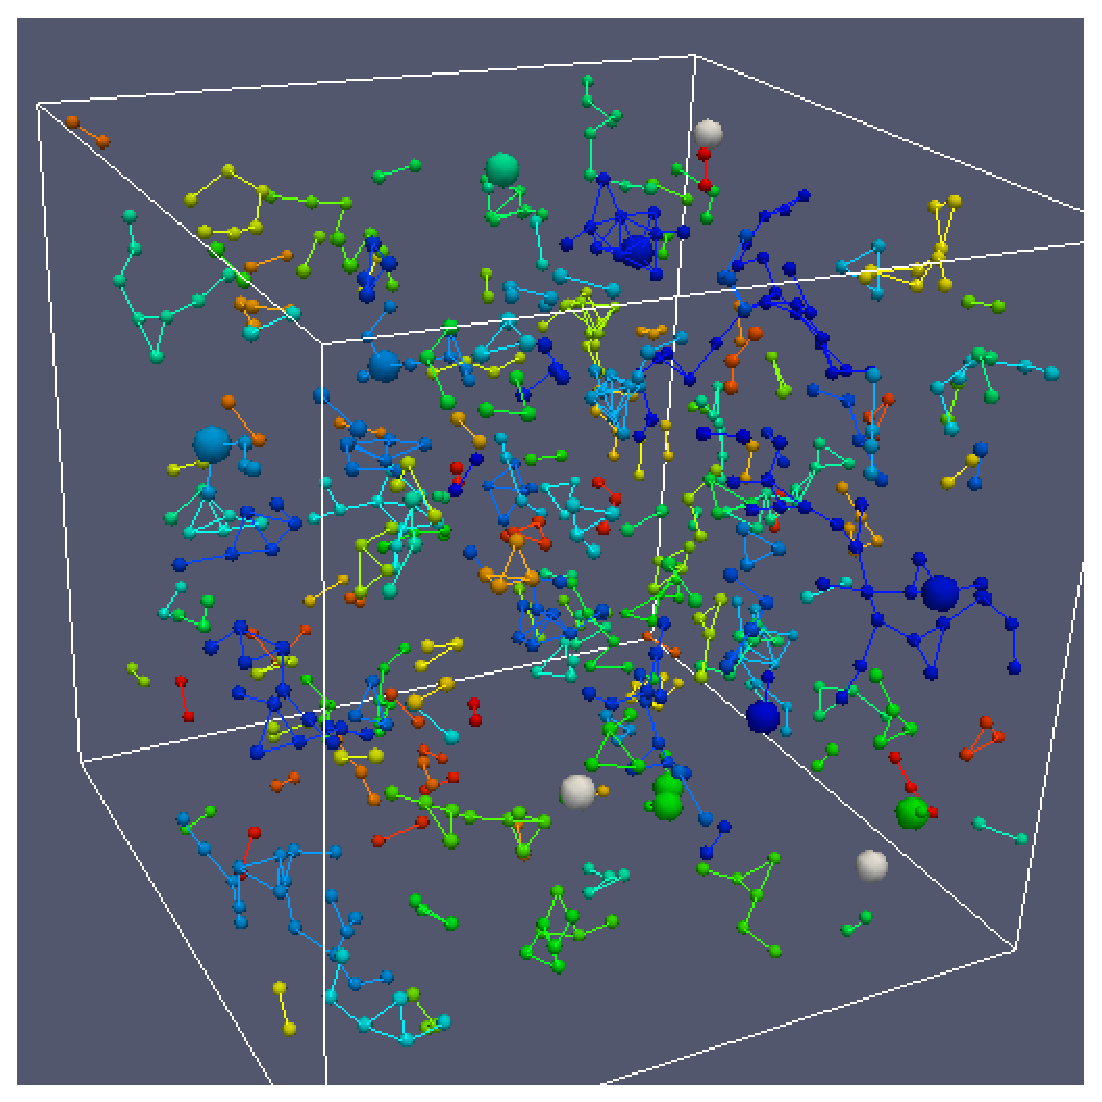
\includegraphics[width=\columnwidth]{stable_ico_4582}
	\[ \phi=0.535 \]}%
	\only<all:3>{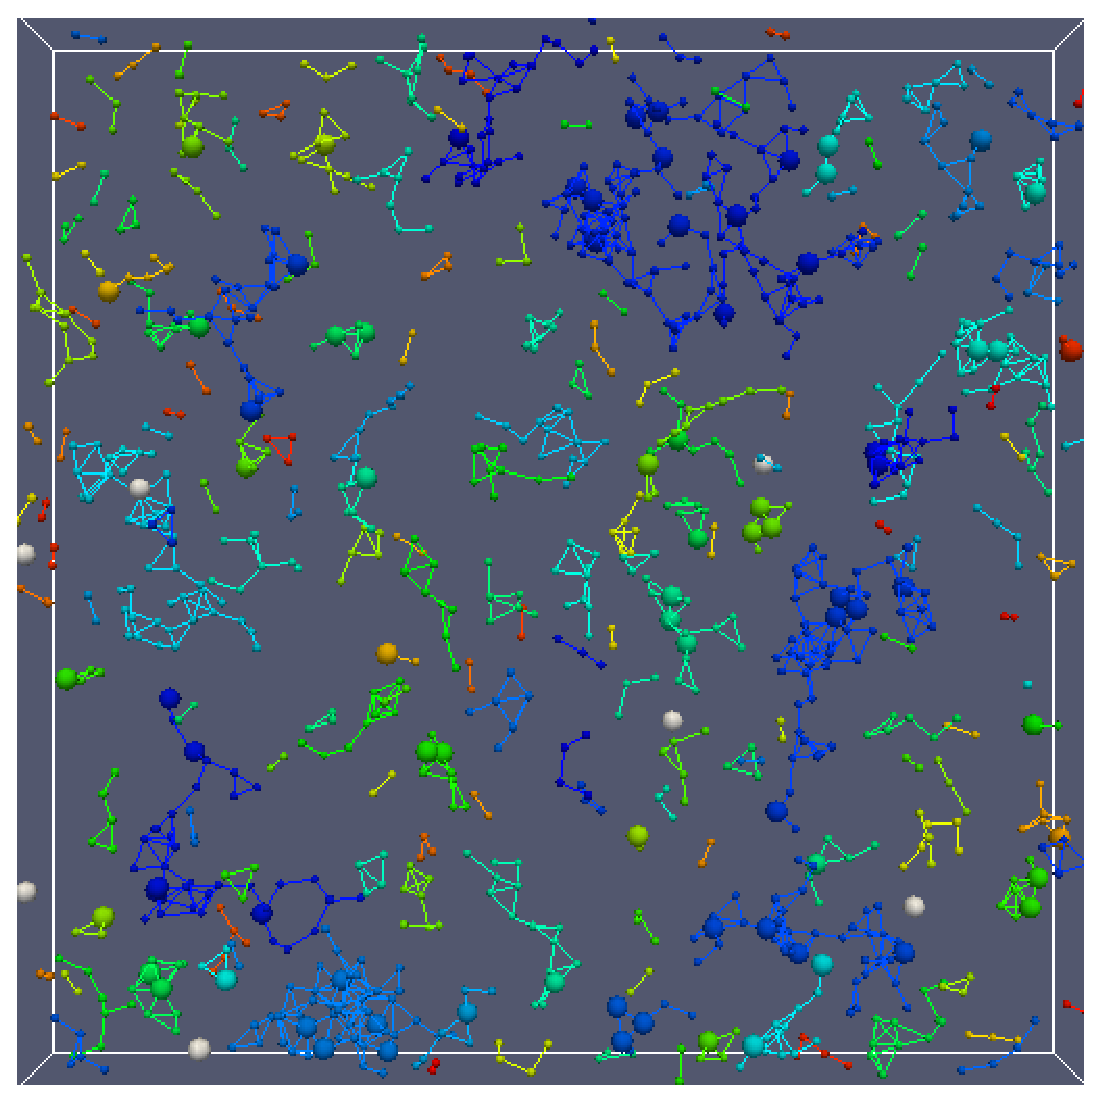
\includegraphics[width=\columnwidth]{stable_ico_go1}
	\[ \phi=0.576 \]}%
	\column{0.4\textwidth}
	\begin{block}{Central particle}
	\begin{itemize}
		\item Perfect \tikz\shade[ball color=gray] (0,0) circle (0.5em);
		\item Imperfect \tikz\shade[ball color=gray] (0,0) circle (0.3em);
	\end{itemize}
	\end{block}
	\begin{itemize}
		\item Perfect icosahedra are few 
		\item No medium range size without the imperfect icosahedra
	\end{itemize}
	\end{columns}
\end{frame}

\begin{frame}{Size of the crystal-like ordered regions}
	\begin{textblock*}{0.6\textwidth}(10mm,92mm)
		\simplephasediagram{}
	\end{textblock*}
	\centering\resizebox{0.5\textwidth}{!}{\begin{LARGE}% GNUPLOT: LaTeX picture with Postscript
\begingroup
  \makeatletter
  \providecommand\color[2][]{%
    \GenericError{(gnuplot) \space\space\space\@spaces}{%
      Package color not loaded in conjunction with
      terminal option `colourtext'%
    }{See the gnuplot documentation for explanation.%
    }{Either use 'blacktext' in gnuplot or load the package
      color.sty in LaTeX.}%
    \renewcommand\color[2][]{}%
  }%
  \providecommand\includegraphics[2][]{%
    \GenericError{(gnuplot) \space\space\space\@spaces}{%
      Package graphicx or graphics not loaded%
    }{See the gnuplot documentation for explanation.%
    }{The gnuplot epslatex terminal needs graphicx.sty or graphics.sty.}%
    \renewcommand\includegraphics[2][]{}%
  }%
  \providecommand\rotatebox[2]{#2}%
  \@ifundefined{ifGPcolor}{%
    \newif\ifGPcolor
    \GPcolortrue
  }{}%
  \@ifundefined{ifGPblacktext}{%
    \newif\ifGPblacktext
    \GPblacktexttrue
  }{}%
  % define a \g@addto@macro without @ in the name:
  \let\gplgaddtomacro\g@addto@macro
  % define empty templates for all commands taking text:
  \gdef\gplbacktext{}%
  \gdef\gplfronttext{}%
  \makeatother
  \ifGPblacktext
    % no textcolor at all
    \def\colorrgb#1{}%
    \def\colorgray#1{}%
  \else
    % gray or color?
    \ifGPcolor
      \def\colorrgb#1{\color[rgb]{#1}}%
      \def\colorgray#1{\color[gray]{#1}}%
      \expandafter\def\csname LTw\endcsname{\color{white}}%
      \expandafter\def\csname LTb\endcsname{\color{black}}%
      \expandafter\def\csname LTa\endcsname{\color{black}}%
      \expandafter\def\csname LT0\endcsname{\color[rgb]{1,0,0}}%
      \expandafter\def\csname LT1\endcsname{\color[rgb]{0,1,0}}%
      \expandafter\def\csname LT2\endcsname{\color[rgb]{0,0,1}}%
      \expandafter\def\csname LT3\endcsname{\color[rgb]{1,0,1}}%
      \expandafter\def\csname LT4\endcsname{\color[rgb]{0,1,1}}%
      \expandafter\def\csname LT5\endcsname{\color[rgb]{1,1,0}}%
      \expandafter\def\csname LT6\endcsname{\color[rgb]{0,0,0}}%
      \expandafter\def\csname LT7\endcsname{\color[rgb]{1,0.3,0}}%
      \expandafter\def\csname LT8\endcsname{\color[rgb]{0.5,0.5,0.5}}%
    \else
      % gray
      \def\colorrgb#1{\color{black}}%
      \def\colorgray#1{\color[gray]{#1}}%
      \expandafter\def\csname LTw\endcsname{\color{white}}%
      \expandafter\def\csname LTb\endcsname{\color{black}}%
      \expandafter\def\csname LTa\endcsname{\color{black}}%
      \expandafter\def\csname LT0\endcsname{\color{black}}%
      \expandafter\def\csname LT1\endcsname{\color{black}}%
      \expandafter\def\csname LT2\endcsname{\color{black}}%
      \expandafter\def\csname LT3\endcsname{\color{black}}%
      \expandafter\def\csname LT4\endcsname{\color{black}}%
      \expandafter\def\csname LT5\endcsname{\color{black}}%
      \expandafter\def\csname LT6\endcsname{\color{black}}%
      \expandafter\def\csname LT7\endcsname{\color{black}}%
      \expandafter\def\csname LT8\endcsname{\color{black}}%
    \fi
  \fi
  \setlength{\unitlength}{0.0500bp}%
  \begin{picture}(7200.00,5040.00)%
    \gplgaddtomacro\gplbacktext{%
      \csname LTb\endcsname%
      \put(1056,704){\makebox(0,0)[r]{\strut{}$10^{-7}$}}%
      \put(1056,1518){\makebox(0,0)[r]{\strut{}$10^{-6}$}}%
      \put(1056,2333){\makebox(0,0)[r]{\strut{}$10^{-5}$}}%
      \put(1056,3147){\makebox(0,0)[r]{\strut{}$10^{-4}$}}%
      \put(1056,3962){\makebox(0,0)[r]{\strut{}$10^{-3}$}}%
      \put(1056,4776){\makebox(0,0)[r]{\strut{}$10^{-2}$}}%
      \put(1453,484){\makebox(0,0){\strut{}$2$}}%
      \put(2117,484){\makebox(0,0){\strut{}$2.5$}}%
      \put(2780,484){\makebox(0,0){\strut{}$3$}}%
      \put(3443,484){\makebox(0,0){\strut{}$3.5$}}%
      \put(4107,484){\makebox(0,0){\strut{}$4$}}%
      \put(4770,484){\makebox(0,0){\strut{}$4.5$}}%
      \put(5433,484){\makebox(0,0){\strut{}$5$}}%
      \put(6097,484){\makebox(0,0){\strut{}$5.5$}}%
      \put(6760,484){\makebox(0,0){\strut{}$6$}}%
      \put(286,2740){\rotatebox{-270}{\makebox(0,0){\strut{}$G_6(r)$}}}%
      \put(6979,2740){\rotatebox{-270}{\makebox(0,0){\strut{}}}}%
      \put(3974,154){\makebox(0,0){\strut{}$r/\sigma$}}%
      \put(3974,4666){\makebox(0,0){\strut{}}}%
      \put(3974,4665){\makebox(0,0){\strut{}}}%
      \put(-264,110){\makebox(0,0)[l]{\strut{}}}%
    }%
    \gplgaddtomacro\gplfronttext{%
      \csname LTb\endcsname%
      \put(2904,932){\makebox(0,0)[r]{\strut{}$\phi=0.535$}}%
      \csname LTb\endcsname%
      \put(2904,1262){\makebox(0,0)[r]{\strut{}$\phi=0.555$}}%
      \csname LTb\endcsname%
      \put(2904,1592){\makebox(0,0)[r]{\strut{}$\phi=0.576$}}%
    }%
    \gplbacktext
    \put(0,0){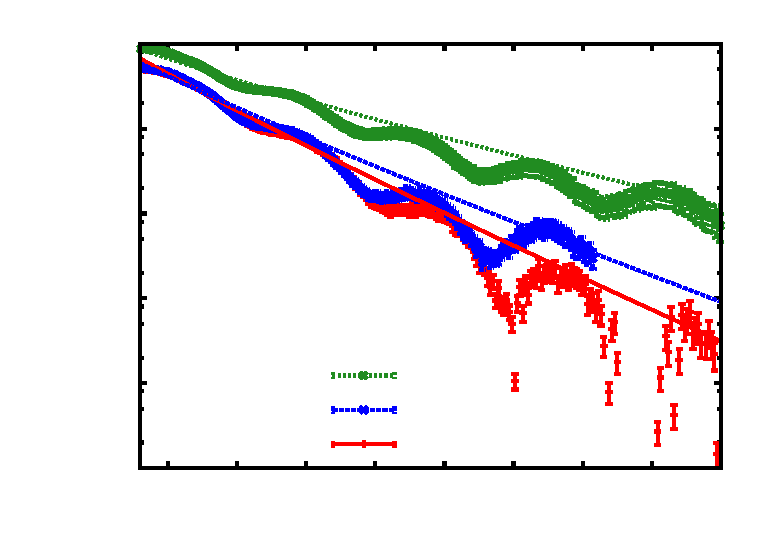
\includegraphics{fit_G6}}%
    \gplfronttext
  \end{picture}%
\endgroup
\end{LARGE}}
	\begin{itemize}
		\item Spatial correlation of the crystal-like order parameter
		\item Ornstein-Zernike fit
		\[ G_6(r) \propto r^{-1}\exp( -\frac{r}{\xi_6} )\]
		\item Growing correlation length
	\end{itemize}
\end{frame}